\section{$t\bar{t}W$ process}
\label{sec:ttV}


\subsection{Samples}
Two MC generators are compared in this study.
The nominal sample for \ttW production was generated using the \textsc{Sherpa}~2.2.1~\cite{sherpa} generator with the NNPDF3.0 NLO PDF set.
The matrix element (ME) was calculated for up to one additional parton at NLO and up to two partons at LO using
\textsc{Comix}~\cite{Gleisberg:2008fv} and \textsc{OpenLoops}~\cite{Cascioli:2011va}, and merged with the \textsc{Sherpa} parton shower~\cite{Schumann:2007mg} using the \textsc{MePs@Nlo} prescription~\cite{Hoeche:2012yf}.
The choice of renormalisation and factorisation scales is $\mu_R = \mu_F = H_\textrm{T}$/2, where $H_\textrm{T}$ is defined as the scalar sum of the transverse masses $\sqrt{p_\textrm{T}^2+m^2}$ of all final state particles.



Systematic uncertainties due to missing higher-order QCD corrections are estimated by varying the factorisation and renormalisation scales in the nominal sample simultaneously by a factor of 0.5 and 2.0 with respect to the central value. 
Uncertainties associated with the modelling of additional QCD radiation are estimated by comparing the nominal \ttW prediction with that of an alternative sample that was generated at NLO with the \textsc{MadGraph5\_aMC@NLO}~2.2.1 generator using the same scale choice and PDF set as for the nominal sample, and interfaced to \textsc{Pythia}~8.2 in combination with the A14 tune. 
The samples configurations are summarised in Table~\ref{tab:mcconfig}.
%%%%%%%%%%%%%%%%%%%%%%%%%%%%%%%%%%%%%%%%
\begin{table}
\begin{center}
\caption{\label{tab:mcconfig}
The configurations used for the event generation of \ttW processes.}
\vspace{0.25cm}
{\small
\setlength\tabcolsep{1.5pt}
\begin{tabular}{llllll}
\hline\hline
Process & Generator & ME order & Parton shower & PDF & Tune  \\
%& (alternative) & (alternative) & & \\
\hline
$\ttbar W$  & \textsc{Sherpa 2.2.1} & \textsc{MePs@Nlo} & \textsc{Sherpa} &  NNPDF3.0 NNLO & \textsc{Sherpa} default \\
& \textsc{MG5\_aMC} & NLO & \textsc{Pythia} 8 & NNPDF3.0 NLO & A14   \\
\hline\hline
\end{tabular}
}
\end{center}
\end{table}


% Finally, the uncertainty due to the choice of PDF set is evaluated using the PDF4LHC15 prescription.

\subsection{Fiducial Volume}
Object and event selection is defined at particle-level that closely matches the detector-level described in reference~\cite{ATLAS-CONF-2019-045}. 
Jets are reconstructed from stable particles with a mean lifetime of $\tau > 3\times 10^{-11}$~s, using the anti-$k_t$ algorithm with a radius parameter of $R=0.4$.
Jets are required to satisfy $\pt > 25~\gev$ and $|\eta| < 2.5$.
Jets are matched to $b$-hadrons with $\mathrm{p_{T}>5 GeV}$ by ghost matching~\cite{Cacciari:2008gn} and are referred to as $b$-jets. 
Electrons and muons, referred to as light leptons, are required to be separated from selected jets by $\Delta R>0.4$. 
Hadronically decaying $\tau$ leptons are required to satisfy $\pt > 25~\gev$ and $|\eta| < 2.5$.
Events are selected with exactly two light leptons.
Leptons are required to have $|\eta|< 2.5$ and $\mathrm{p_{T}>25(20) GeV}$ for leading (subleading) lepton. 
Leptons are required to have same charge, targeting the semi-leptonic $\mathrm{t\bar{t}}$ decay and leptonic $W$ decay.

%Events separated by Hadronic tau decays Hadronically decaying $\tau$ lepton
Events with at least 3 jets and least one $b$-jet are considered in the fiducial volume. 
The acceptance for events passing this selection is $A_X^{\geq1b\geq3j}=1.82\times10^{-2}$ for \textsc{Sherpa} and 1.90$\times10^{-2}$ for \textsc{MadGraph5\_aMC@NLO} correspondingly.
We then split into five regions, categorized by the number of jets (three or  $\geq$4), $b$-jets (one or $\geq$2) as well as the presence of hadronically decaying $\tau$ lepton. 
				\begin{description}
				\item Region 1: 1 $N_{b-jets}$, ~ $\geq$4 $N_{jets}$ , 0-$\tau_{had}$
				\item Region 2: $\geq$2 $N_{b-jets}$,   $\geq$4 $N_{jets}$, 0-$\tau_{had}$
				\item Region 3: 1 $N_{b-jets}$, ~  3 $N_{jets}$ , 0-$\tau_{had}$
				\item Region 4: $\geq$2 $N_{b-jets}$, 3 $N_{jets}$, 0-$\tau_{had}$
				\item Region 5: $\geq$1 $N_{b-jets}$, $\geq$3 $N_{jets}$, 1-$\tau_{had}$
				\end{description}
Definitions of the regions are motivated by $t\bar{t}H$ analysis strategy.
Regions 1 and 2 corresponds to the signal regions\footnote{slightly different then in ~\cite{ATLAS-CONF-2019-045}, in order to define a common selection with the CMS collaboration} and Regions 3 and 4 are used as control regions in the 2$\ell$ same-sign  0-$\tau_{had}$ $t\bar{t}H$ channel.
Definition of Region 5 is closely followed\footnote{requirement on jet multiplicity is relaxed} by the selections in 2$\ell$ same-sign 1-$\tau_{had}$ $t\bar{t}H$ channel.

%The event selection requirements are summarized in Table~\ref{}.
%defined by 5 jets \& 3 b-jets or >=6jets \& >=4 b-jets.




\subsection{Results}

The nominal  \textsc{Sherpa} \ttW  sample is compared to its radiation uncertainty variations and the alternative generator.
The ratio plot shows the ratio of the alternative MC sample and scale variation to the nominal sample.%Discrepancies between PP8 $\mathrm{t\bar{t}}$ and the alternative generators can be seen in the $\Delta R$ quantities\&\ref{ttbb:mindR}, where at least in the 4b selection the difference to the alternative generators is larger than the uncertainty band given by the radiation variations.  
%Interesting differences are also observed in the HT distributions, particularly in the 3b selection, as illustrated in Figures~\ref{ttbb:HTbjets}\&\ref{ttbb:HTljets}. The jet multiplicity, as in Figure~\ref{ttbb:Njets}, has poor agreement among the generators for large jet multiplicities.

Sizeable discrepancies in the modelling of jet kinematics can be seen between the \textsc{Sherpa} \ttW and \textsc{MadGraph5\_aMC@NLO} generators in 1$b$-jet selections, while in $\geq2b$-jets the difference is reduced, as illustrated in Figures~\ref{ttV:4j12b} and~\ref{ttV:3j12b} for the high (Regions 1 and 2) and low (Regions 3 and 4) jet multiplicities correspondingly. 

\begin{figure}[!htb]
\centering
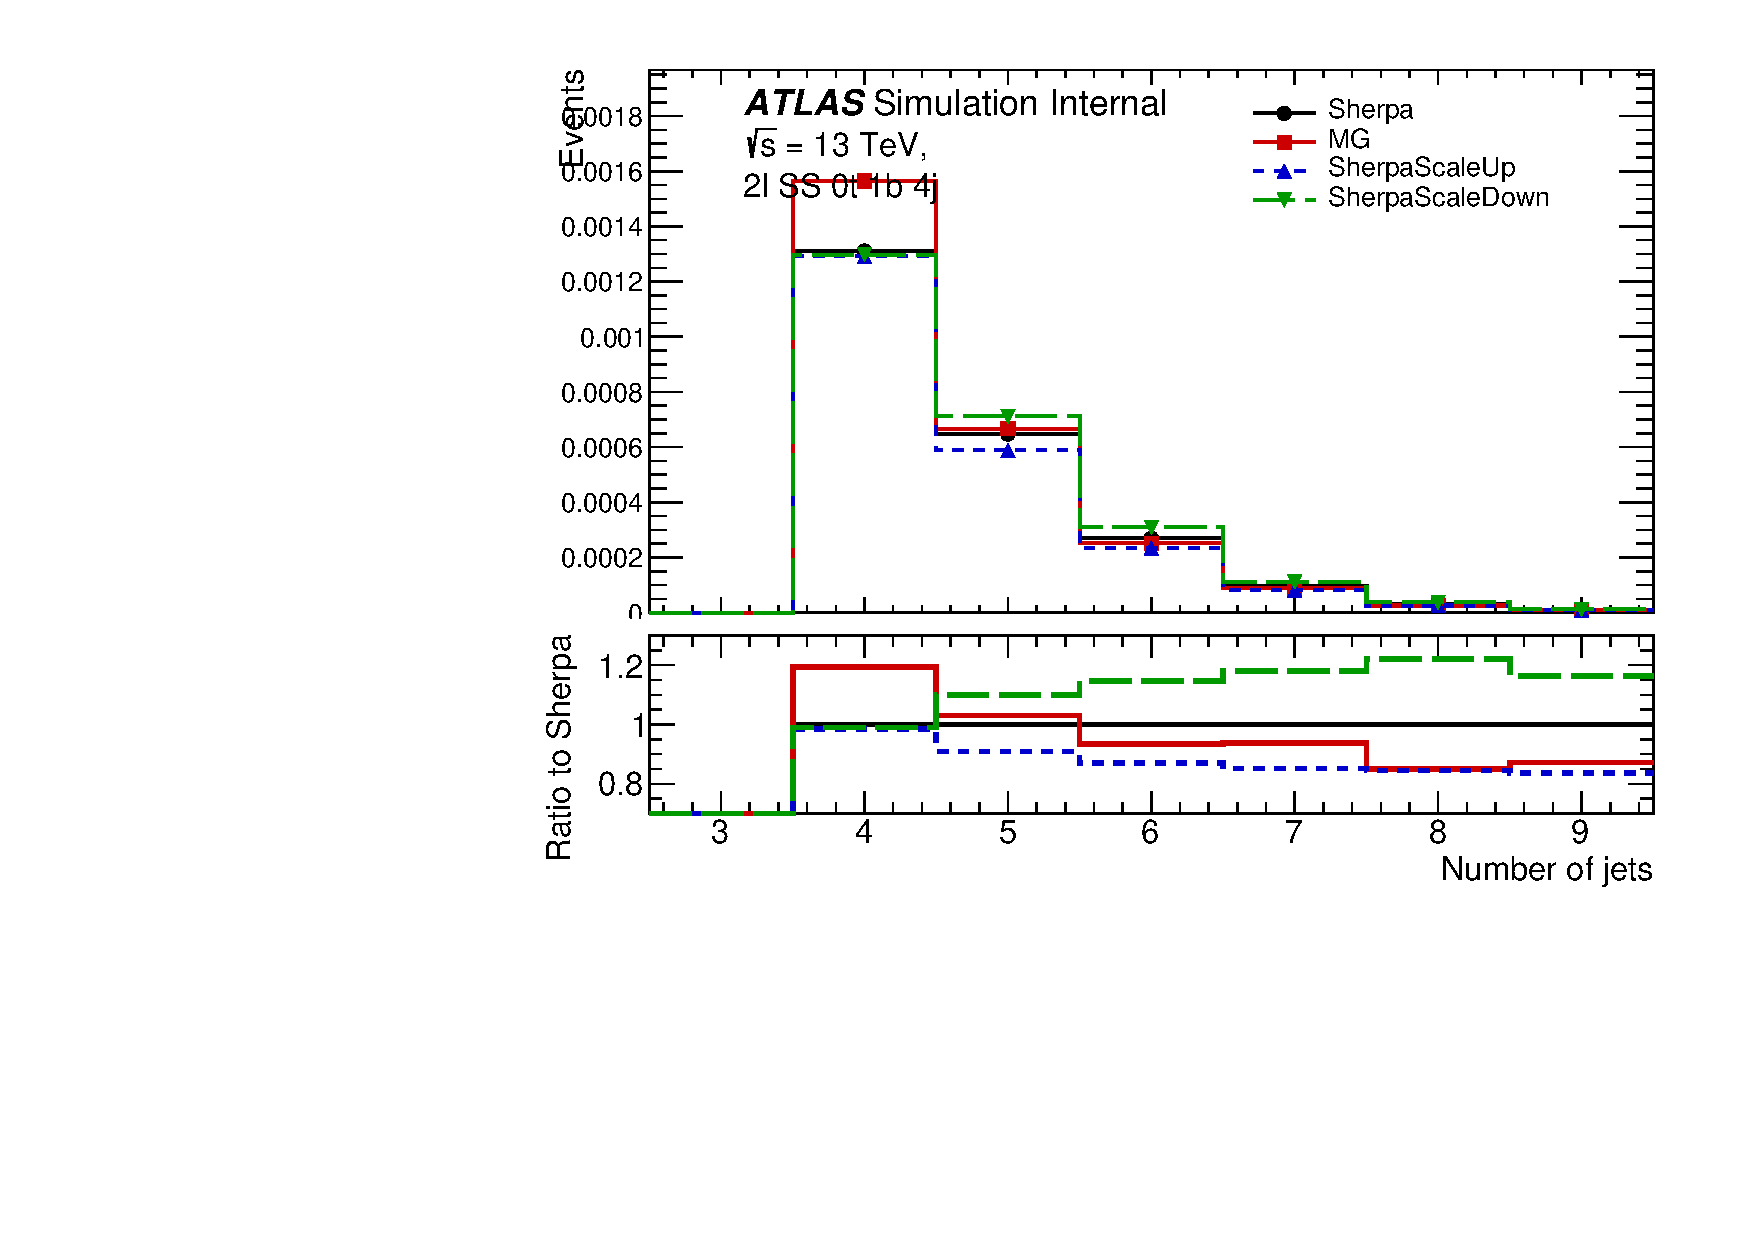
\includegraphics[width=0.45\textwidth]{Plots/ttV/c_Region_0_nJets}
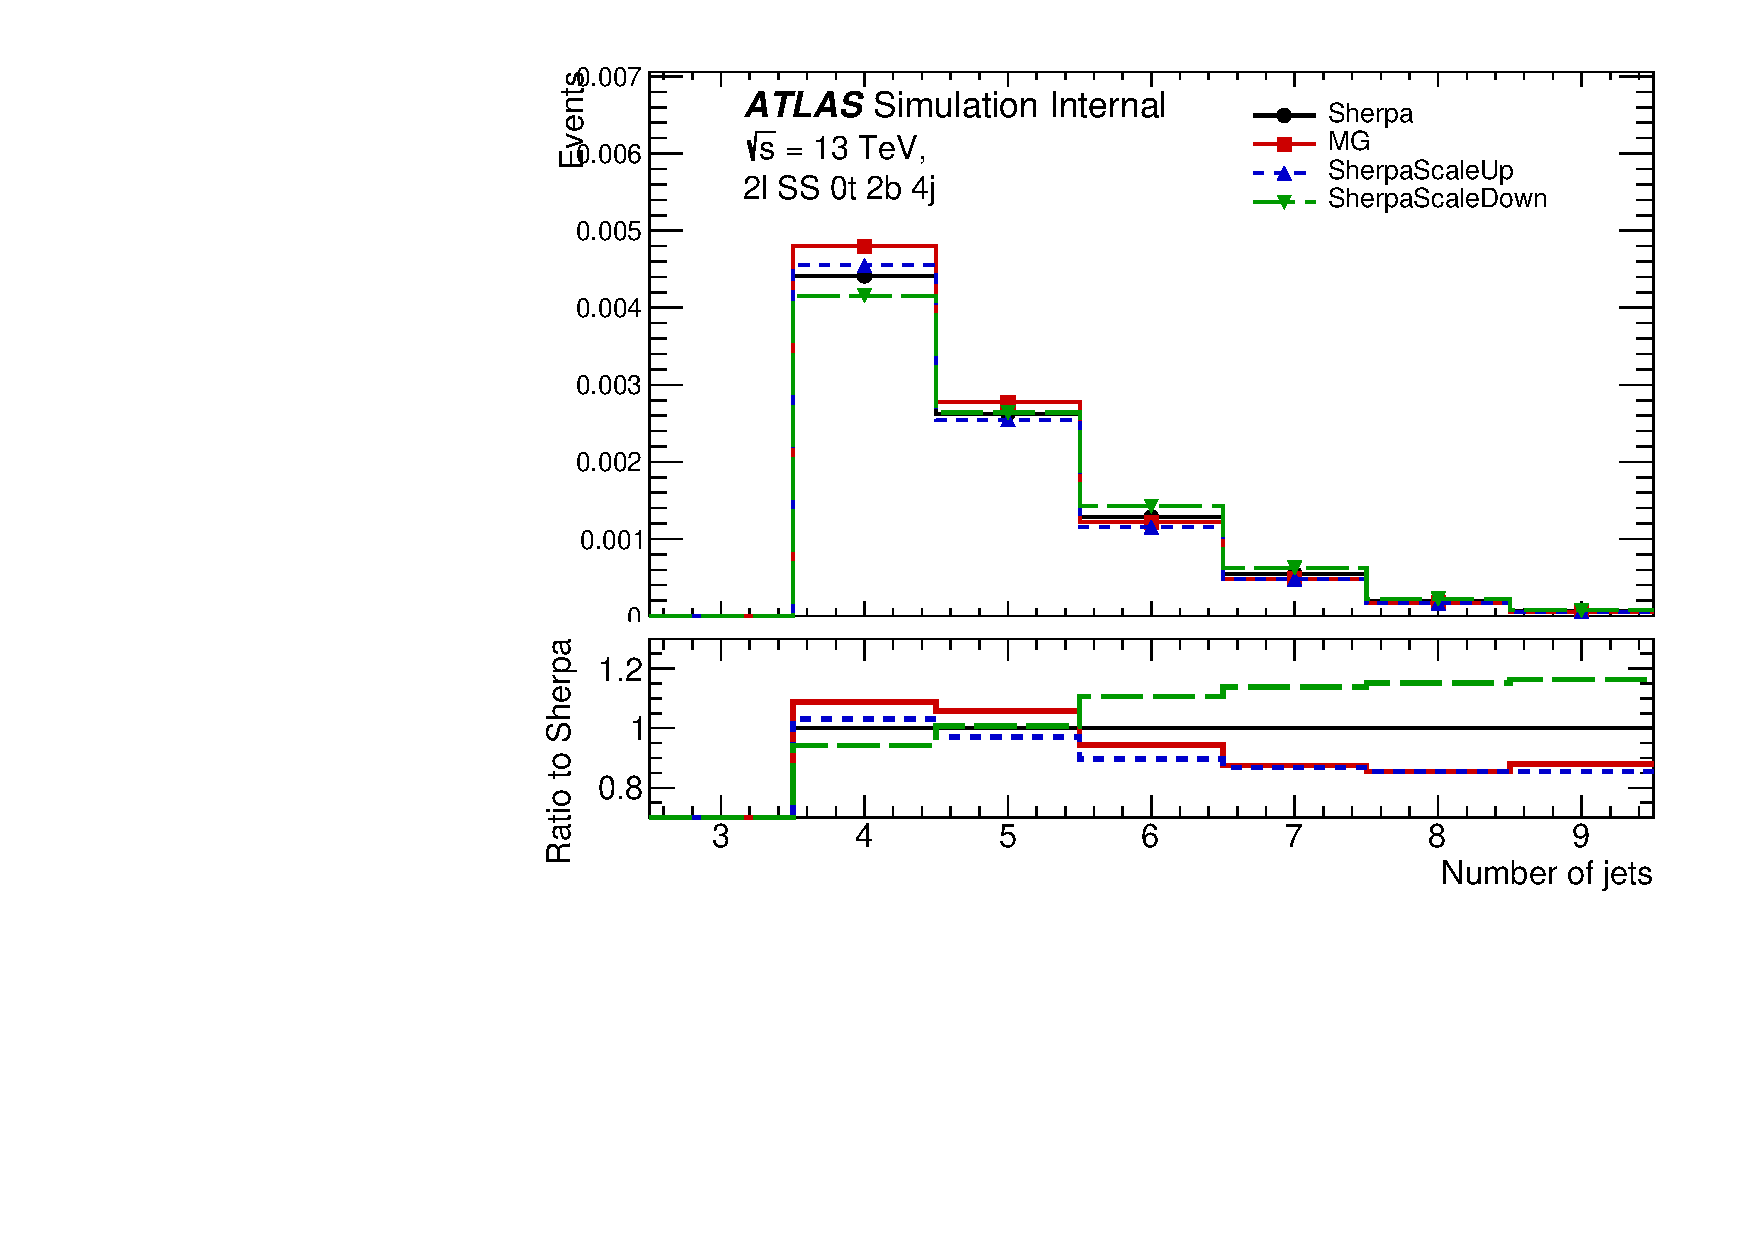
\includegraphics[width=0.45\textwidth]{Plots/ttV/c_Region_1_nJets}\\
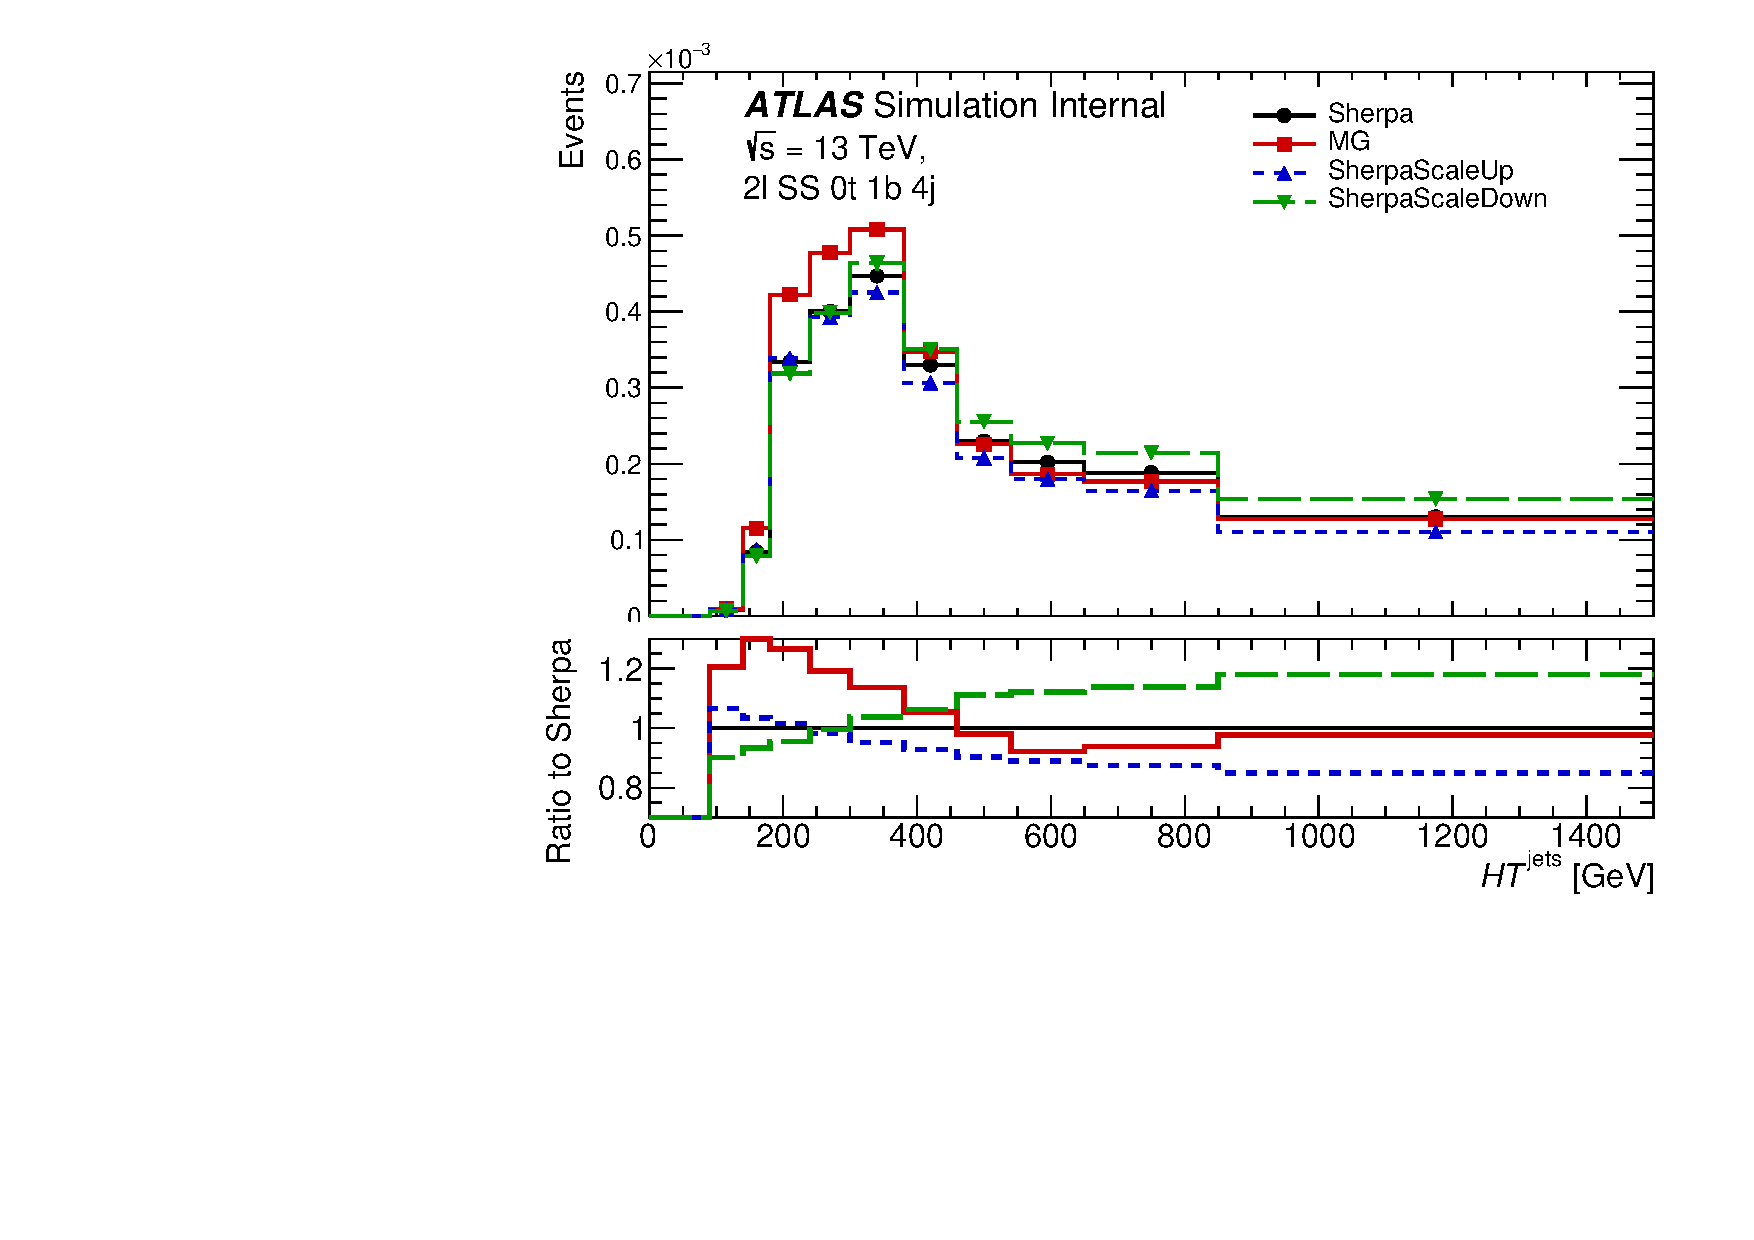
\includegraphics[width=0.45\textwidth]{Plots/ttV/c_Region_0_HT_jets}
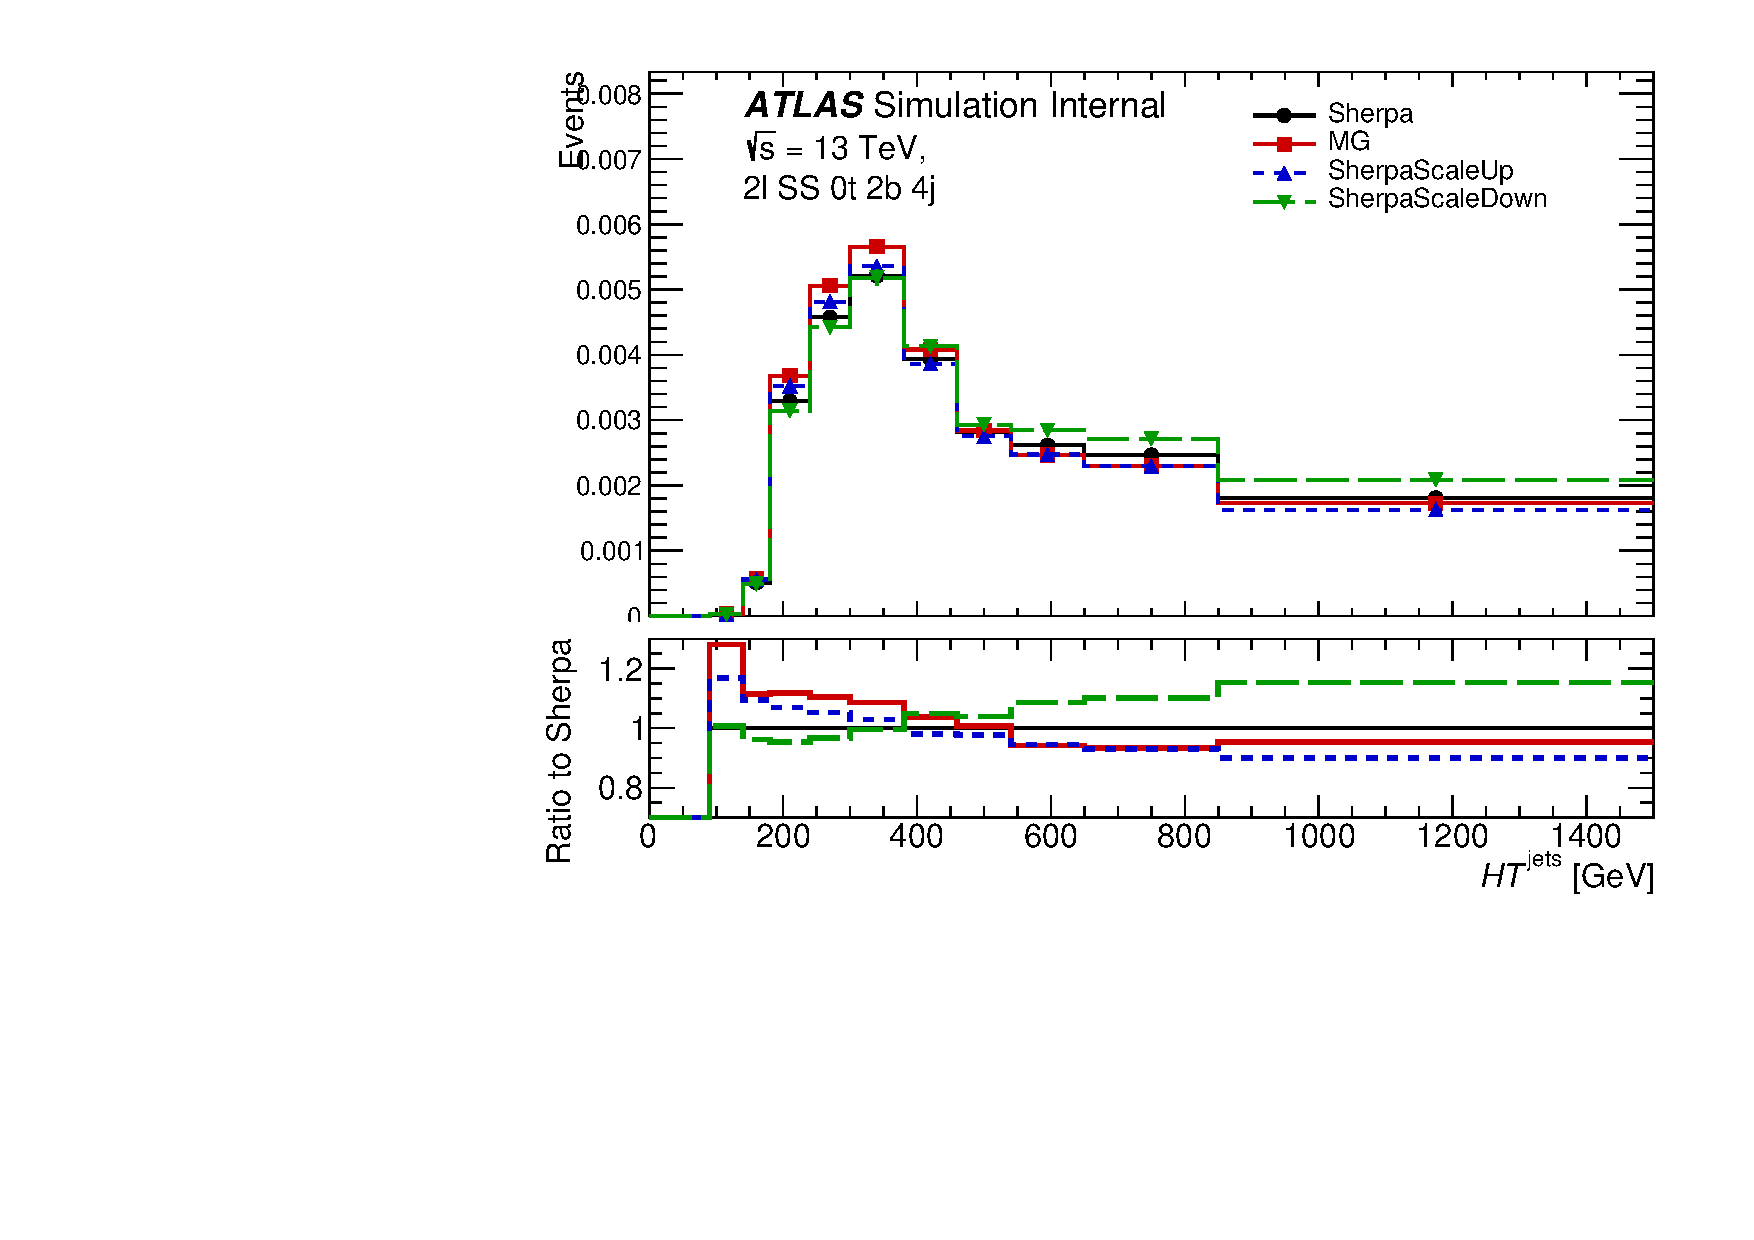
\includegraphics[width=0.45\textwidth]{Plots/ttV/c_Region_1_HT_jets}\\
  \caption{Distribution of the jet multiplicities (top) and the sum of jets transverse momentum, $HT^{\text{jets}}$ (bottom), for the Region 1 with 1$b$-jet (left) and Region 2 with 2$b$-jets (right) selection requiring four and more jets. Explanation in text. \label{ttV:4j12b}}
\end{figure}


\begin{figure}[!htb]
\centering
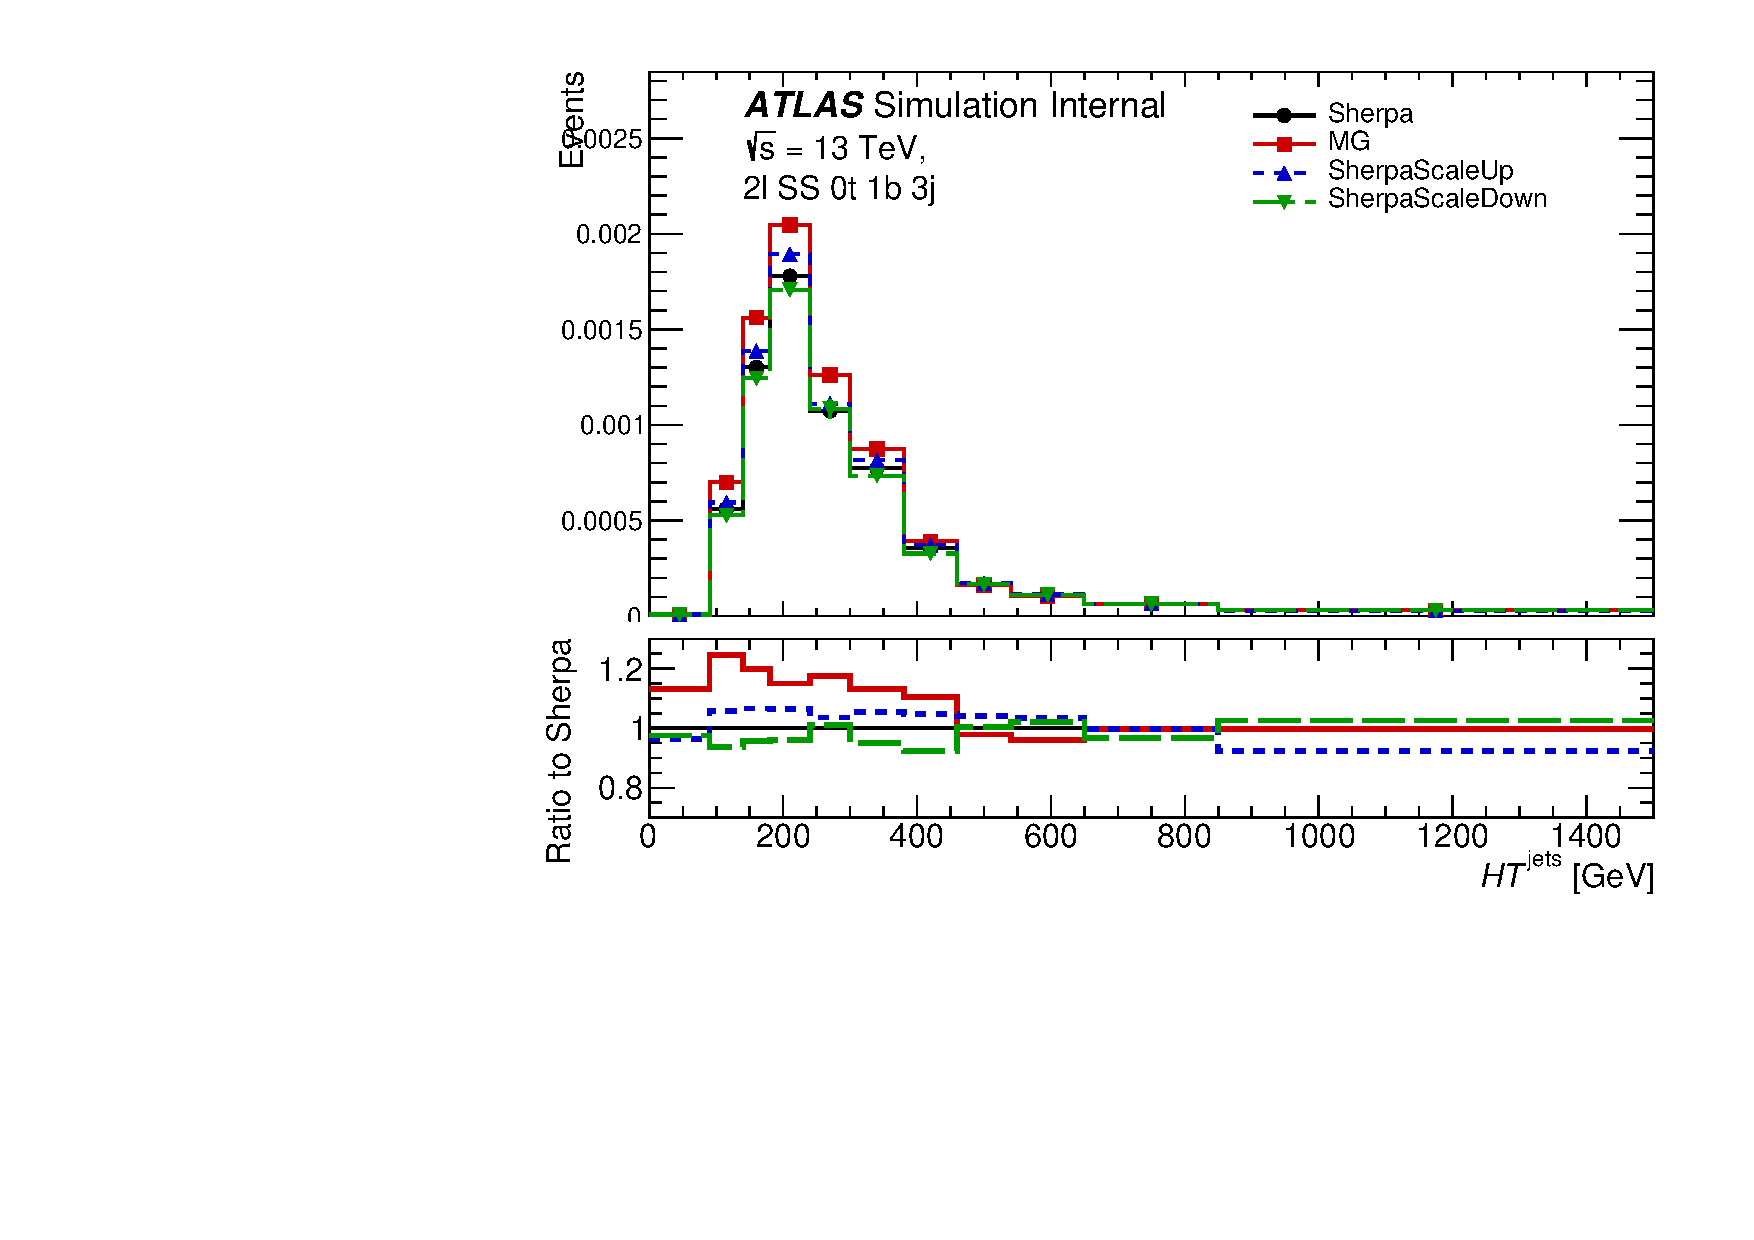
\includegraphics[width=0.45\textwidth]{Plots/ttV/c_Region_2_HT_jets}
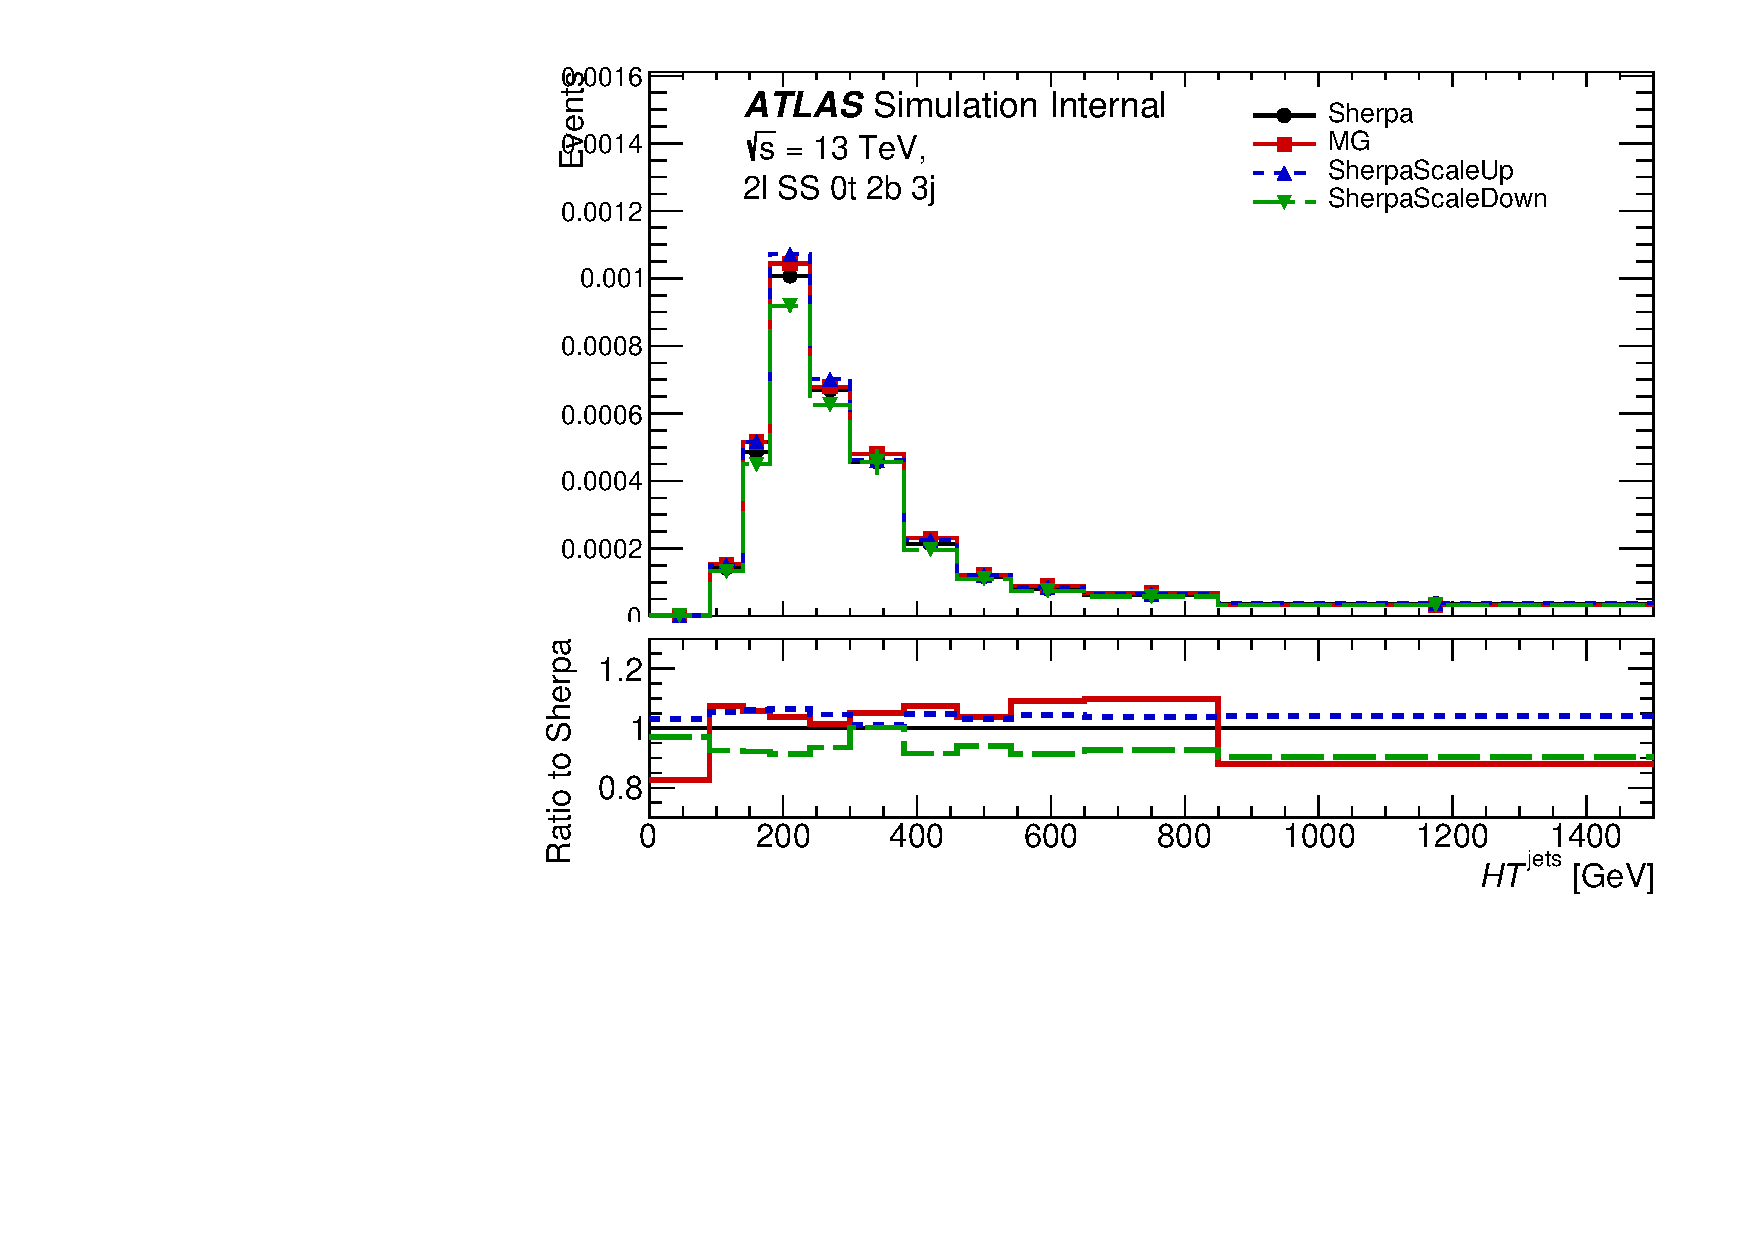
\includegraphics[width=0.45\textwidth]{Plots/ttV/c_Region_3_HT_jets}\\
  \caption{Distribution of the sum of jets transverse momentum, $HT^{\text{jets}}$, for the Region 3 with 1$b$-jet (left) and Region 4 with 2$b$-jets (right) selection requiring exactly three jets. Explanation in text. \label{ttV:3j12b}}
\end{figure}

Good agreement of the single lepton kinematics can be seen between nominal and alternative generators for $\geq2b$-jets selections, as presented in the right of Figures~\ref{ttV:lep_kin} (presented Region 2, while similar behaviour seen in Region 4 as well). 
While there is an offset of the order of 10\%  between nominal and alternative generators for 1$b$-jet selections, as presented in the left of Figures~\ref{ttV:lep_kin} (Region 1 showed, while similar trend seen in Region 3 as well). 

Sizeable difference in shapes between nominal and alternative generators observed for the distributions corresponding to the correlations between two leptons such as the angular distance between the two leptons, maximum of lepton's pseudorapidity and azimuthal separation between the leptons, as illustrated in Figures~\ref{ttV:ll_kin} for Region 1 on the right and Region 2 on the left (similar trends observed in Regions 3 and 4).
As was observed for single lepton kinematics, difference in 1$b$-jet selections is increased wrt to $\geq2b$-jets selection.
%Distributions are presented for $\geq2N_{b-jets},\geq4N_{jets}$ region, while similar behaviour seen in all other regions as well.

Distributions of the jet multiplicity, number of $b$-jets, the leading lepton transverse momentum and the angular distance between the two leptons  $\Delta R _{\ell \ell }$ for the Region 5 with 1$\tau_{had}$ selection are presented on Figure~\ref{ttV:tauR_kin}.
The difference of 10\% observed between nominal and alternative generators for low jet multiplicities, while for $N_{jets}\geq5$ the difference is covered by the scale variation uncertainties. 
The distribution of $b$-jets agrees for $N_{b-jets}$ equal to two, and has sizeable difference in the 1$b$-jet bin, similarly to 0$\tau_{had}$ selections.
Lepton kinematic distributions has difference in shapes between nominal and alternative generators.

\begin{figure}[!htb]
\centering
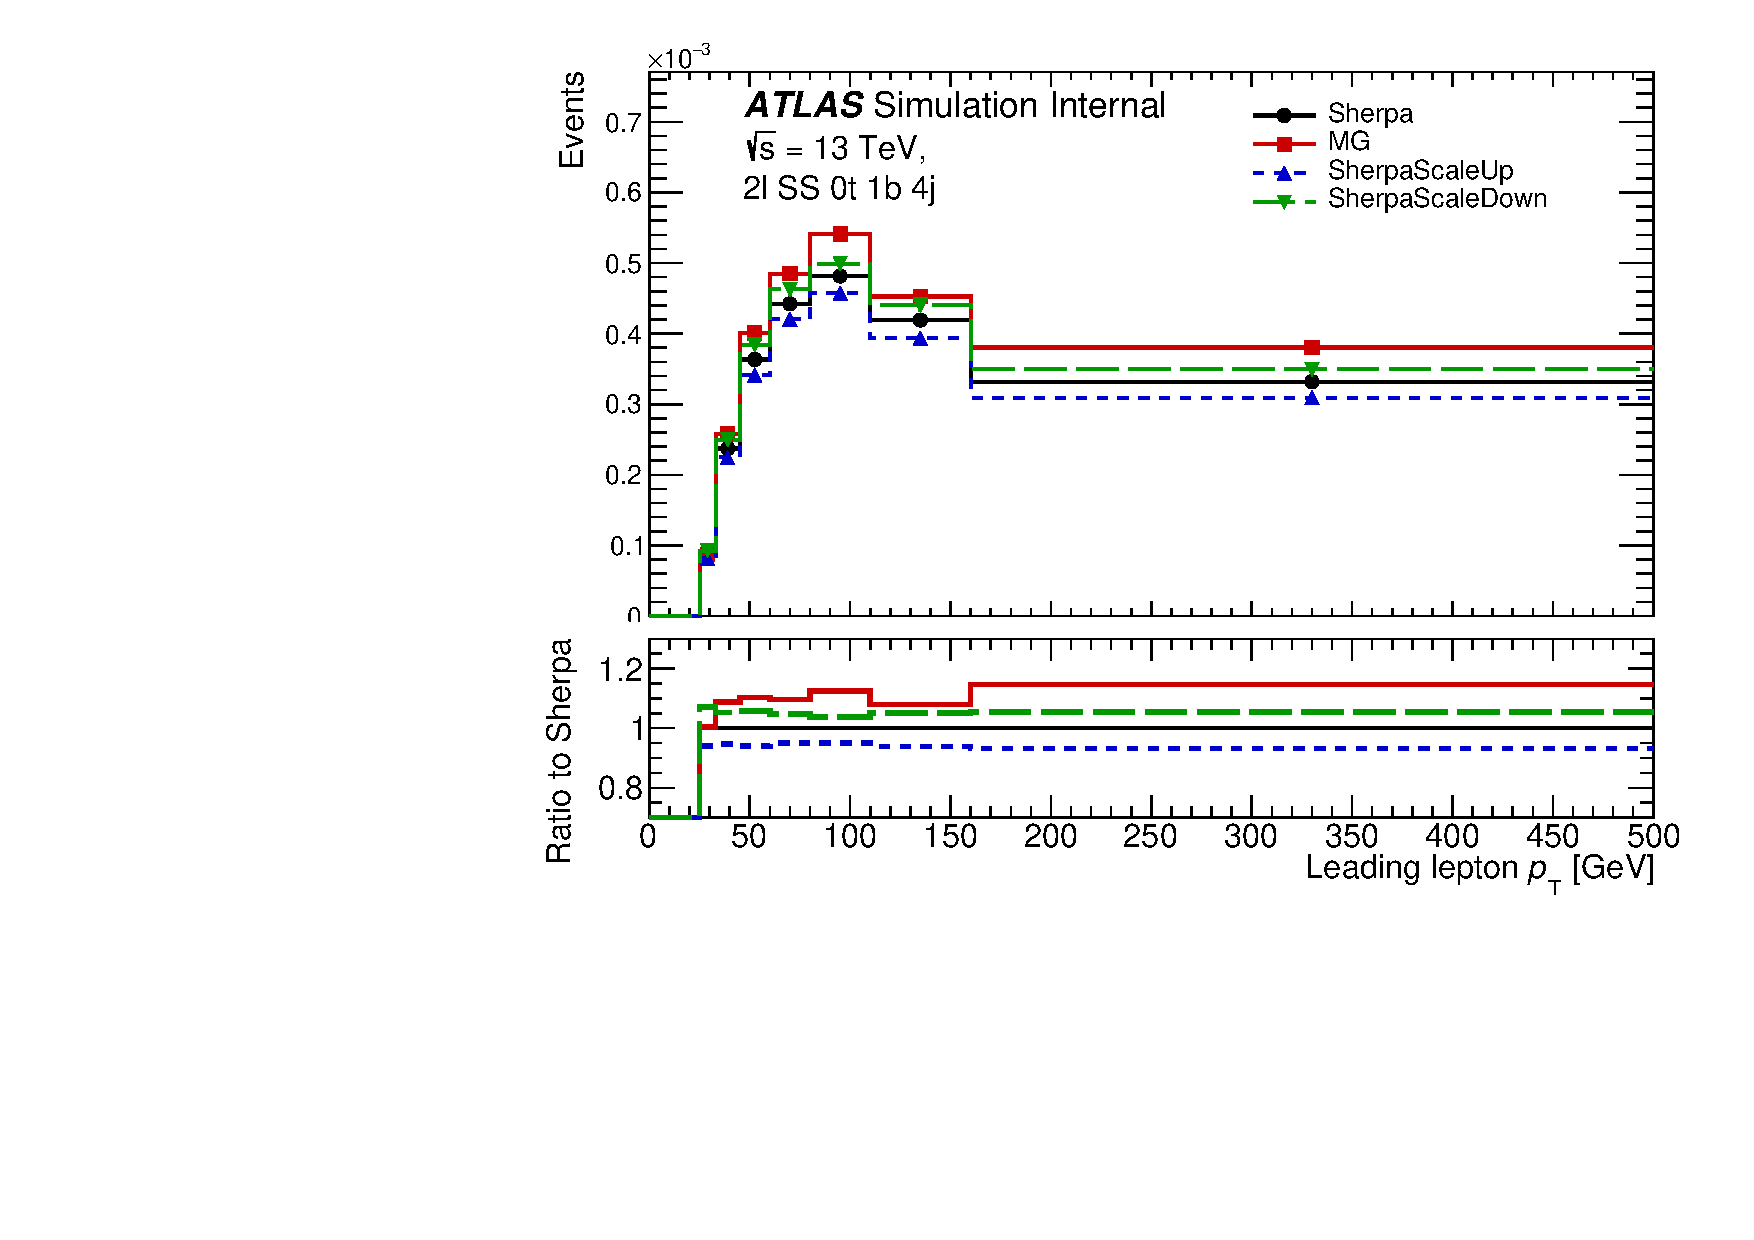
\includegraphics[width=0.45\textwidth]{Plots/ttV/c_Region_0_lep_Pt_0}
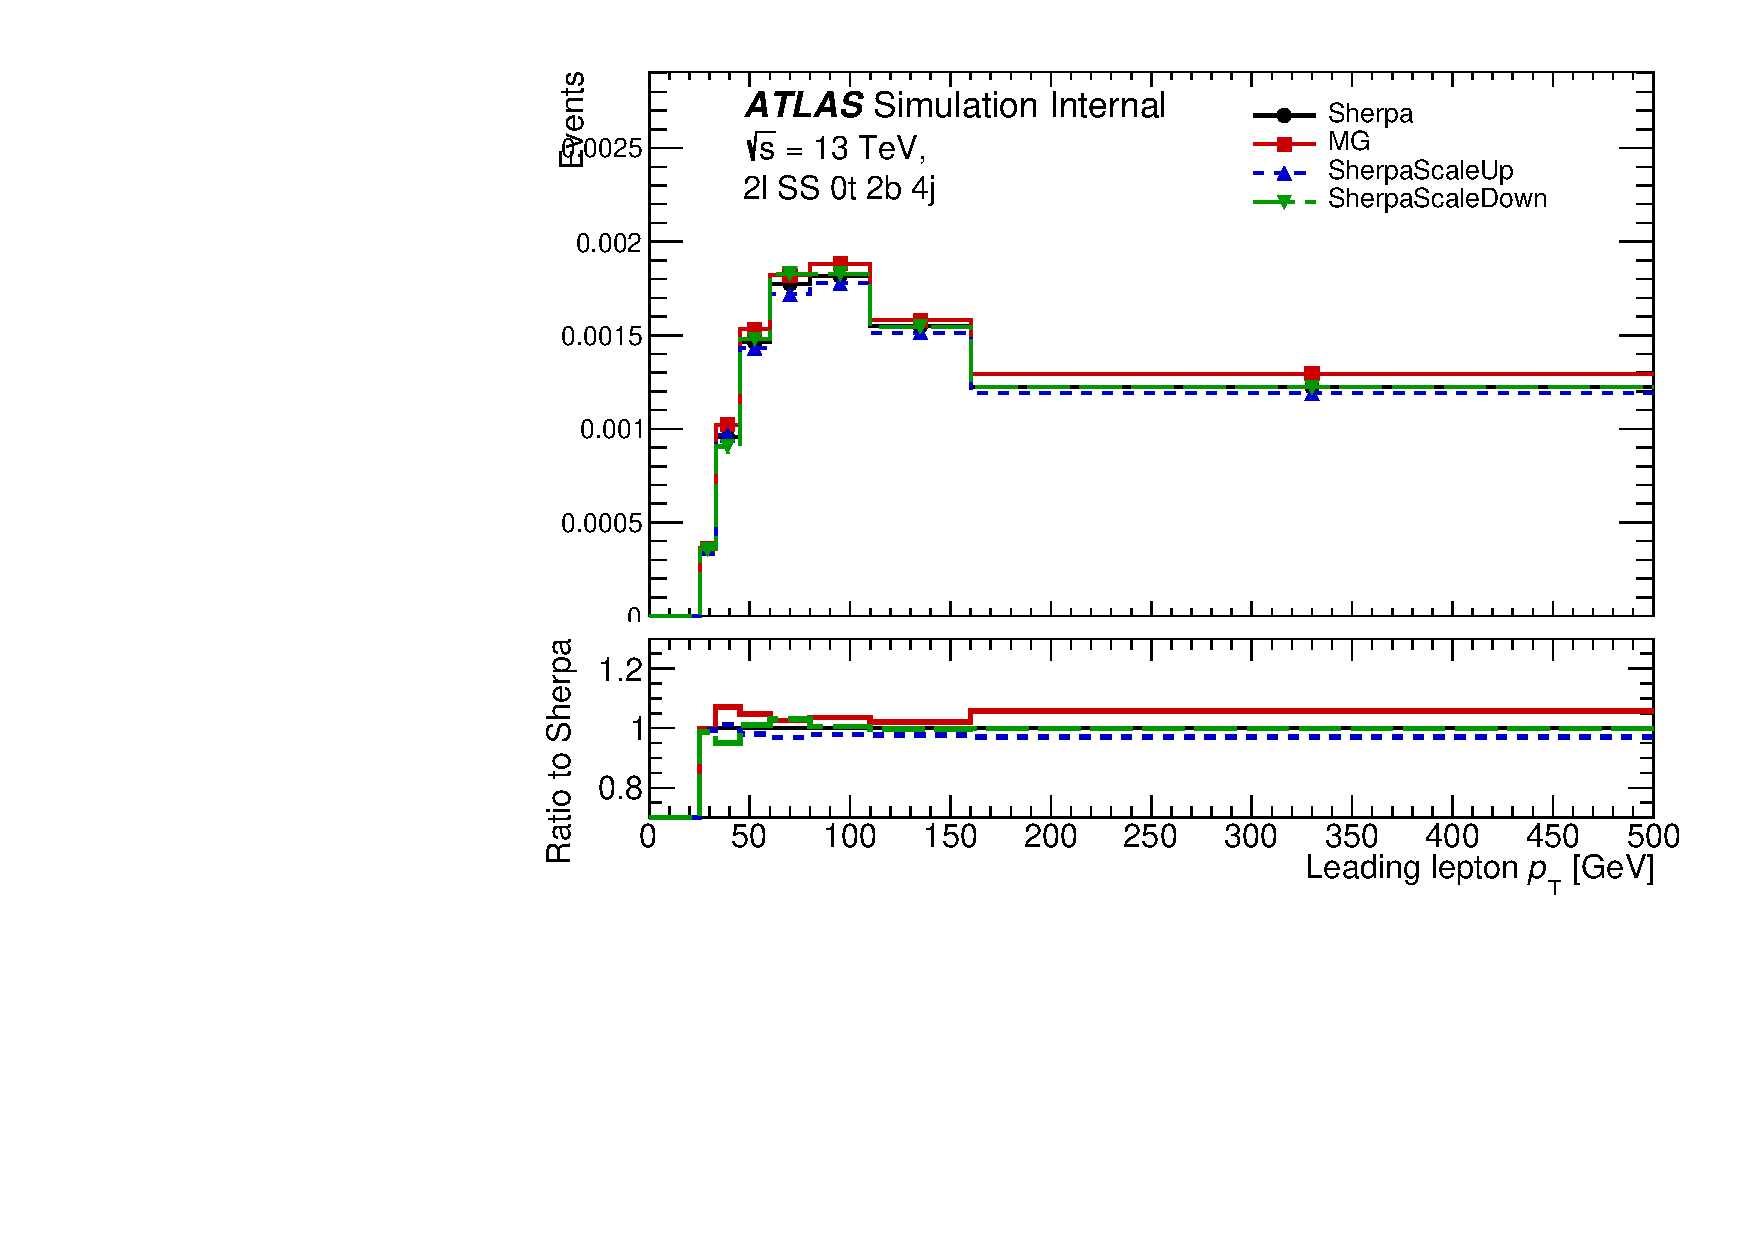
\includegraphics[width=0.45\textwidth]{Plots/ttV/c_Region_1_lep_Pt_0}\\
%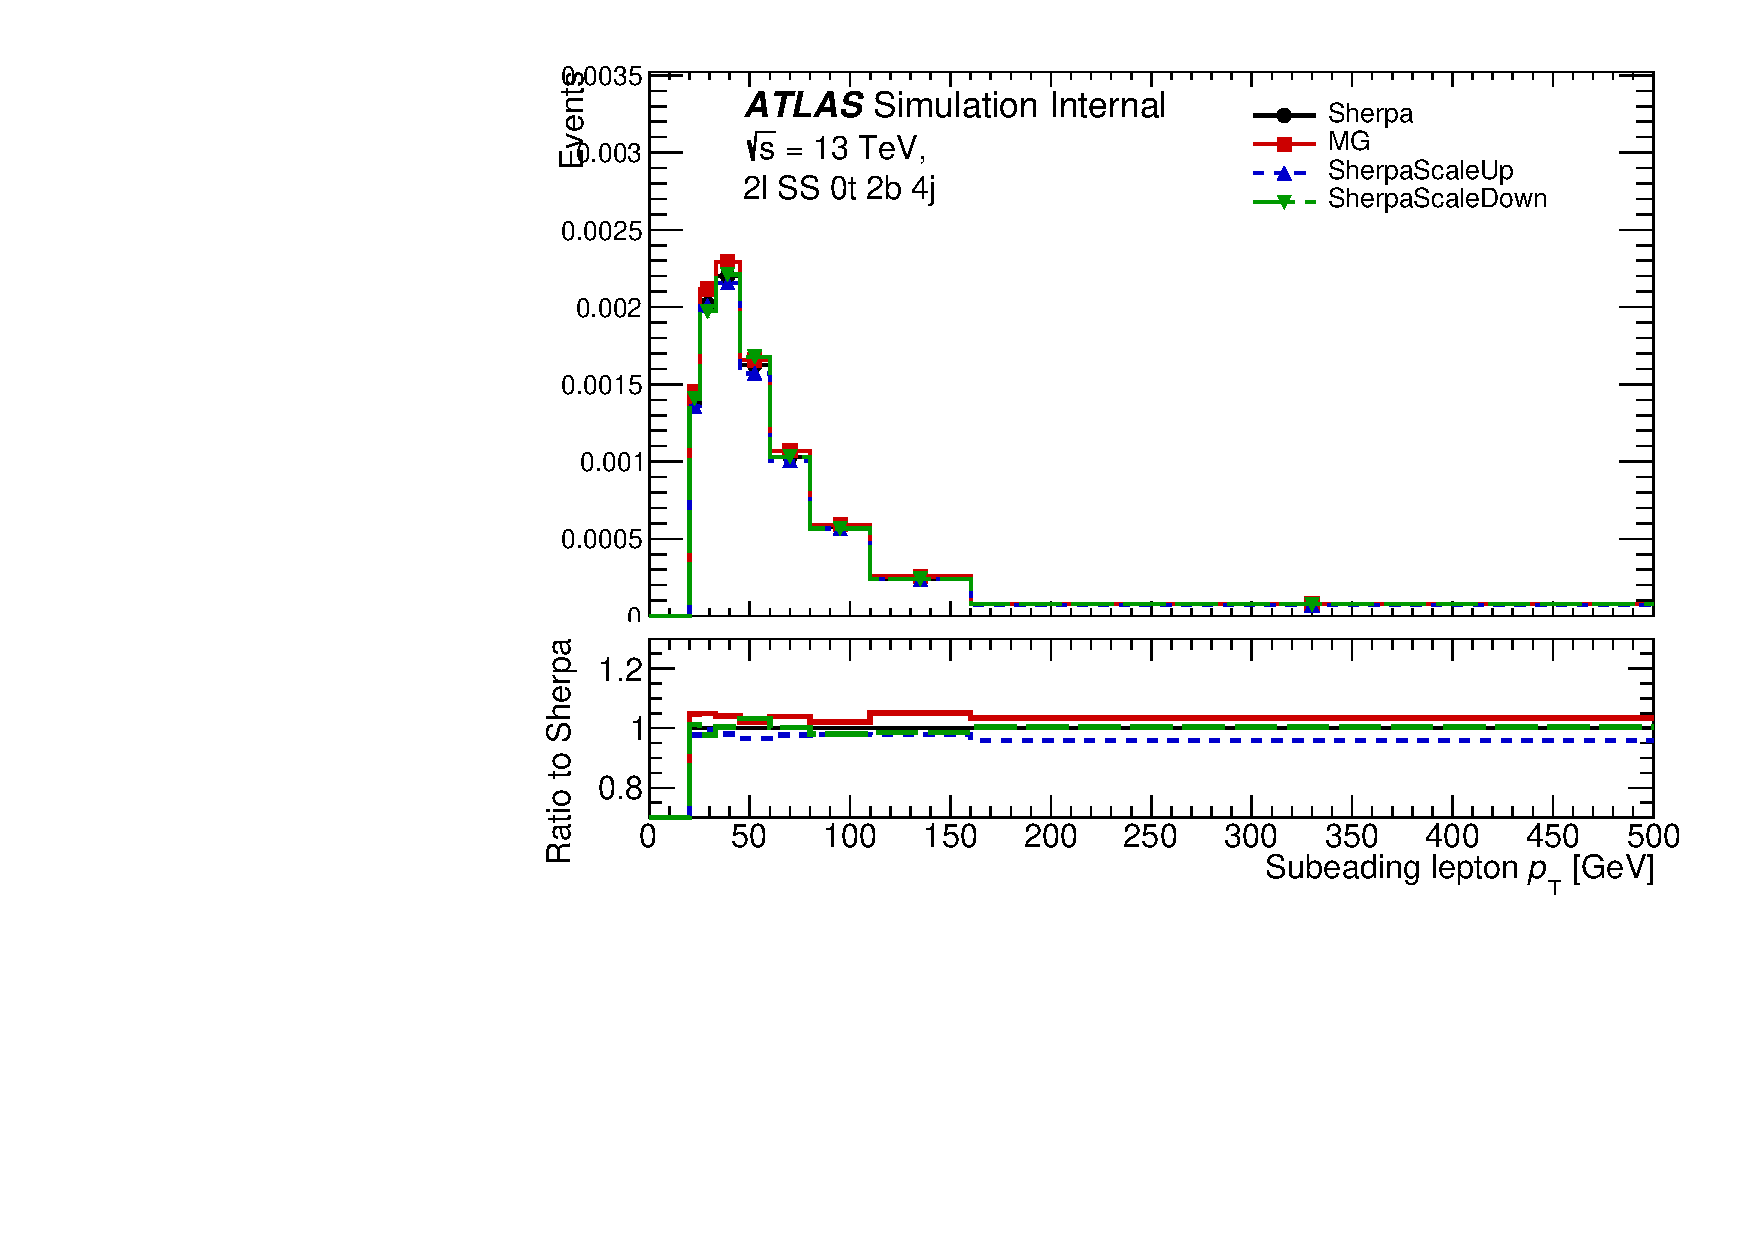
\includegraphics[width=0.45\textwidth]{Plots/ttV/c_Region_1_lep_Pt_1}
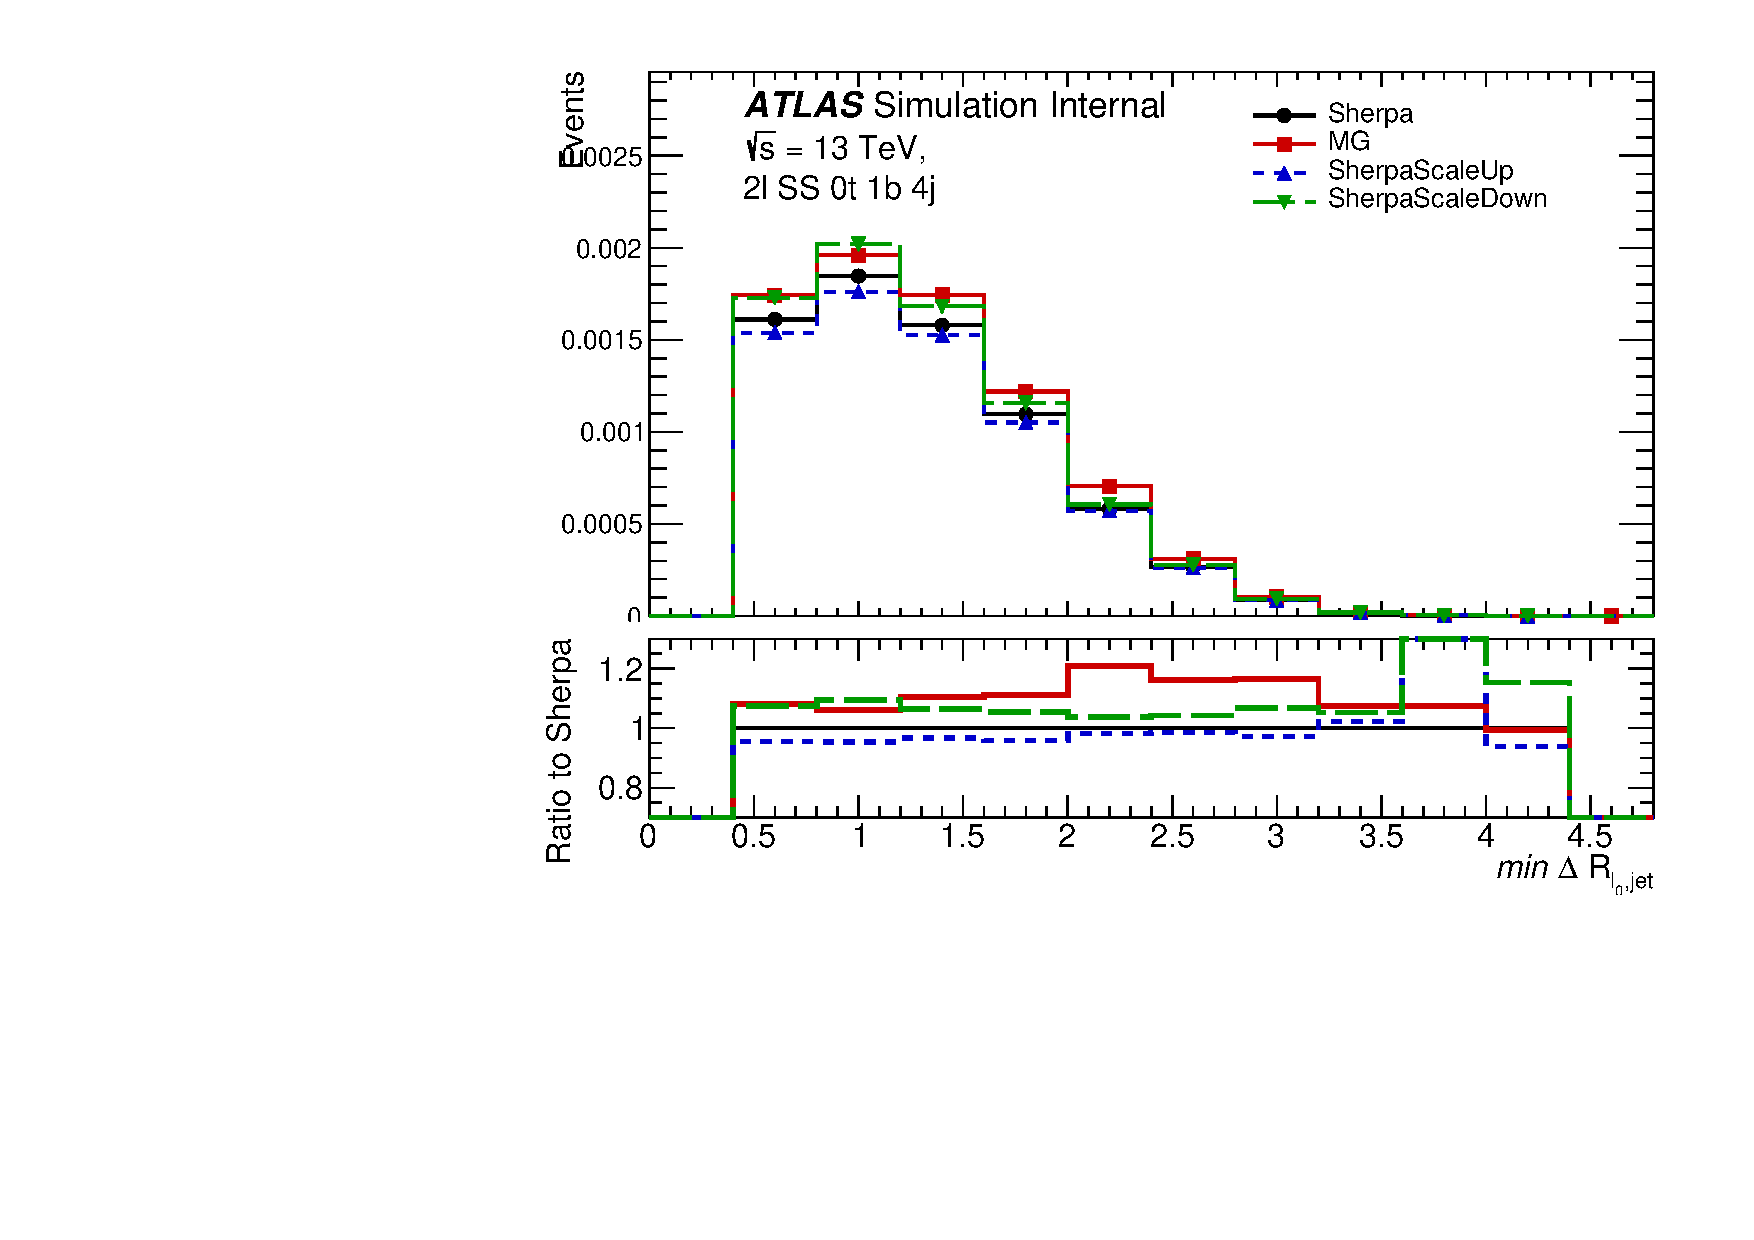
\includegraphics[width=0.45\textwidth]{Plots/ttV/c_Region_0_min_DRl0j}
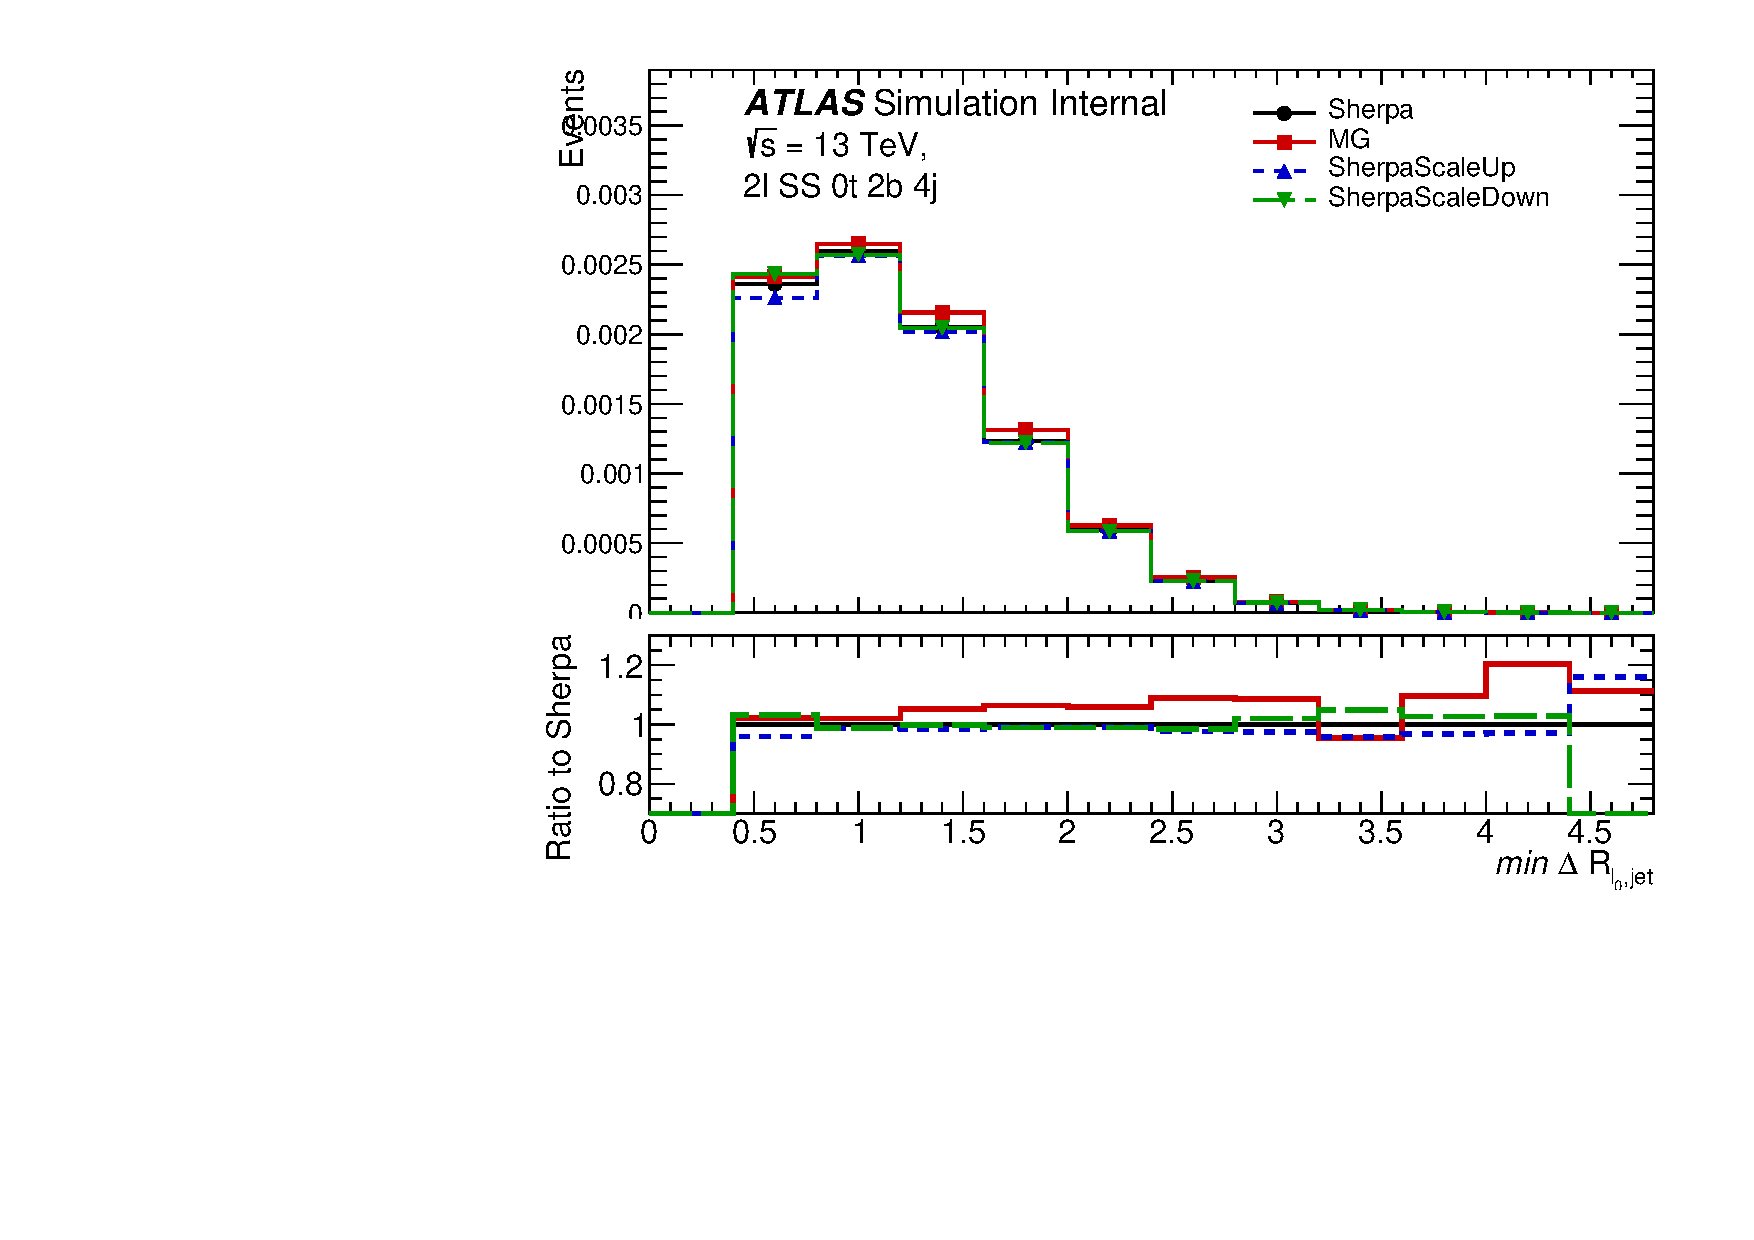
\includegraphics[width=0.45\textwidth]{Plots/ttV/c_Region_1_min_DRl0j}\\
  \caption{Distribution of the leading lepton transverse momentum (top) and the minimum angular separation between the leading lepton and the nearest jet (bottom), for the Region 1 with 1$b$-jet (left) and Region 2 with 2$b$-jets (right) selection requiring four and more jets. Explanation in text.
  \label{ttV:lep_kin}}
\end{figure}

\begin{figure}[!htb]
\centering
	% \hspace{25mm} $DRl_0l_1$  \hspace{20mm} $max|\eta^{\ell\ell}|$\\
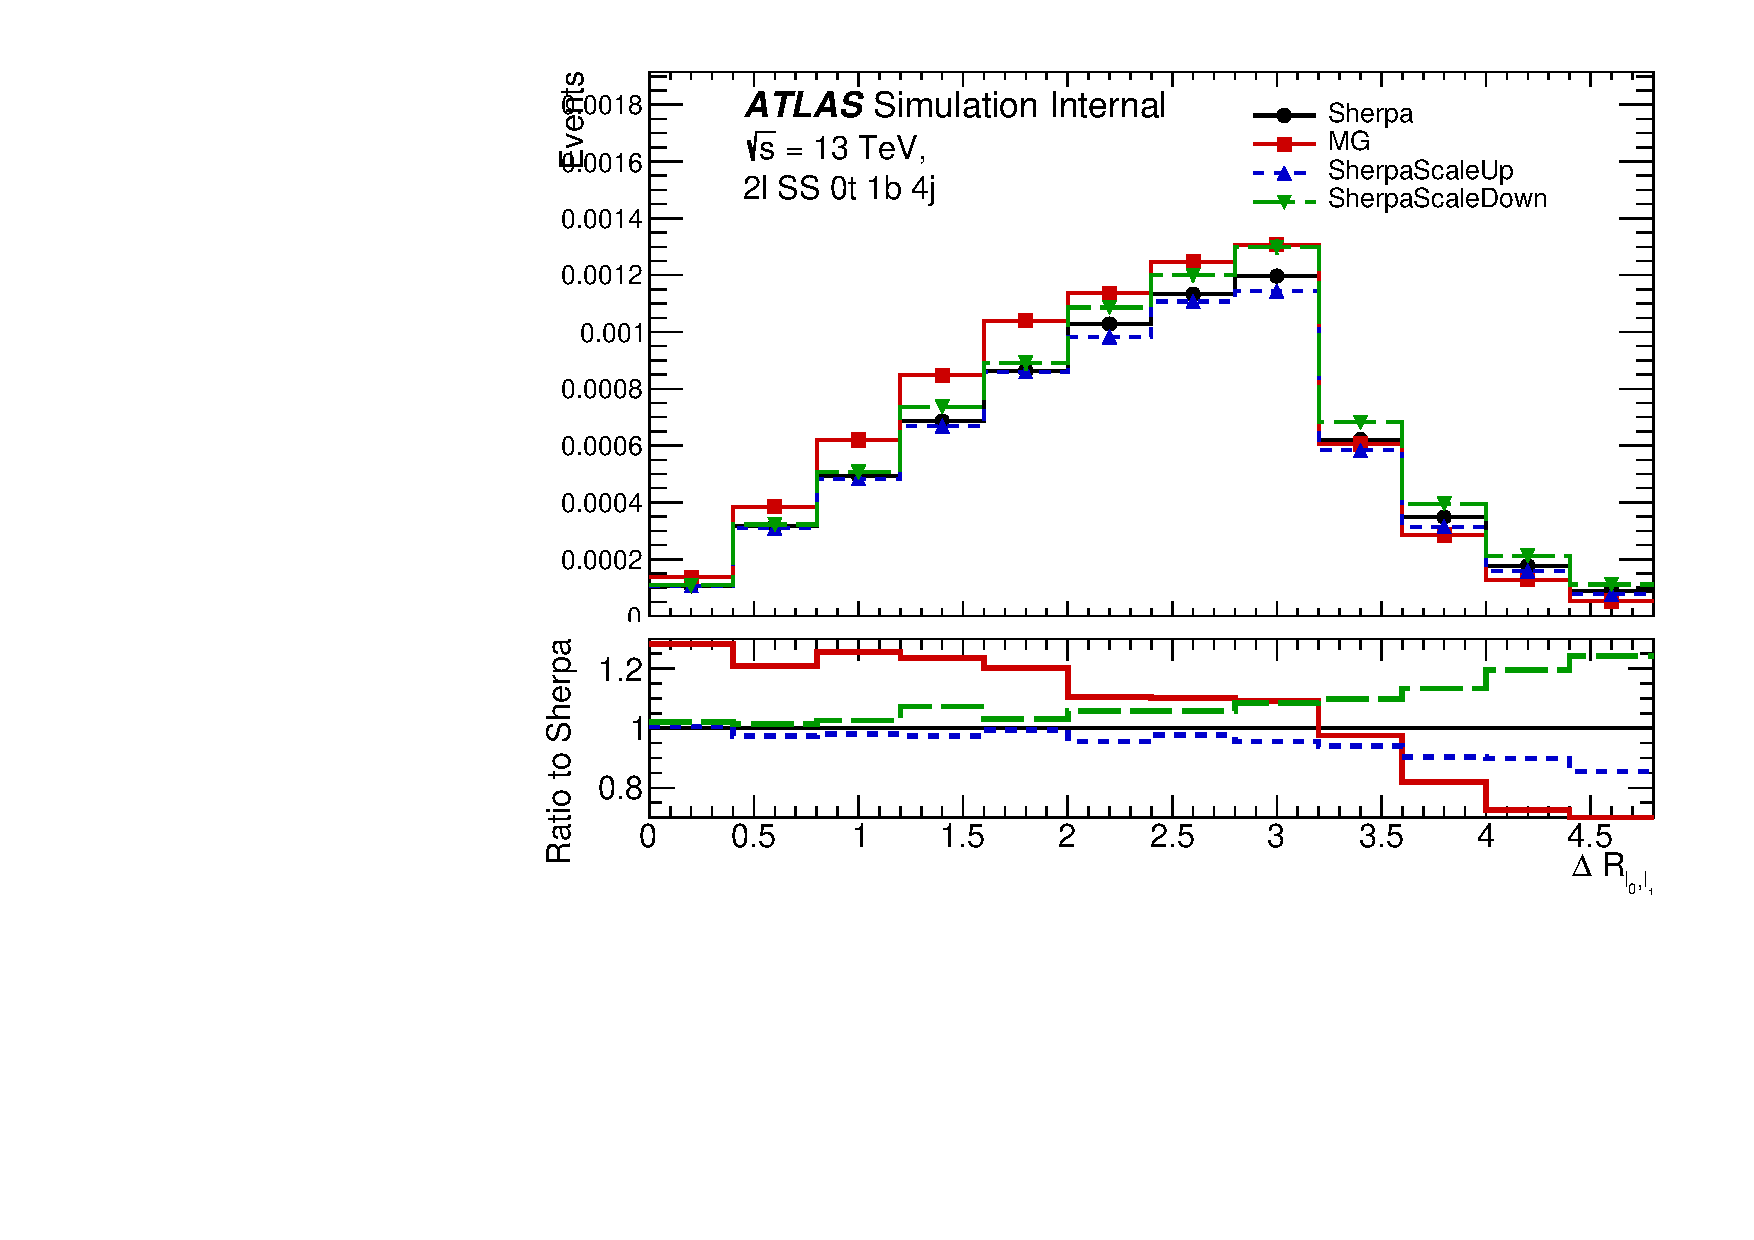
\includegraphics[width=0.45\textwidth]{Plots/ttV/c_Region_0_DRll01}
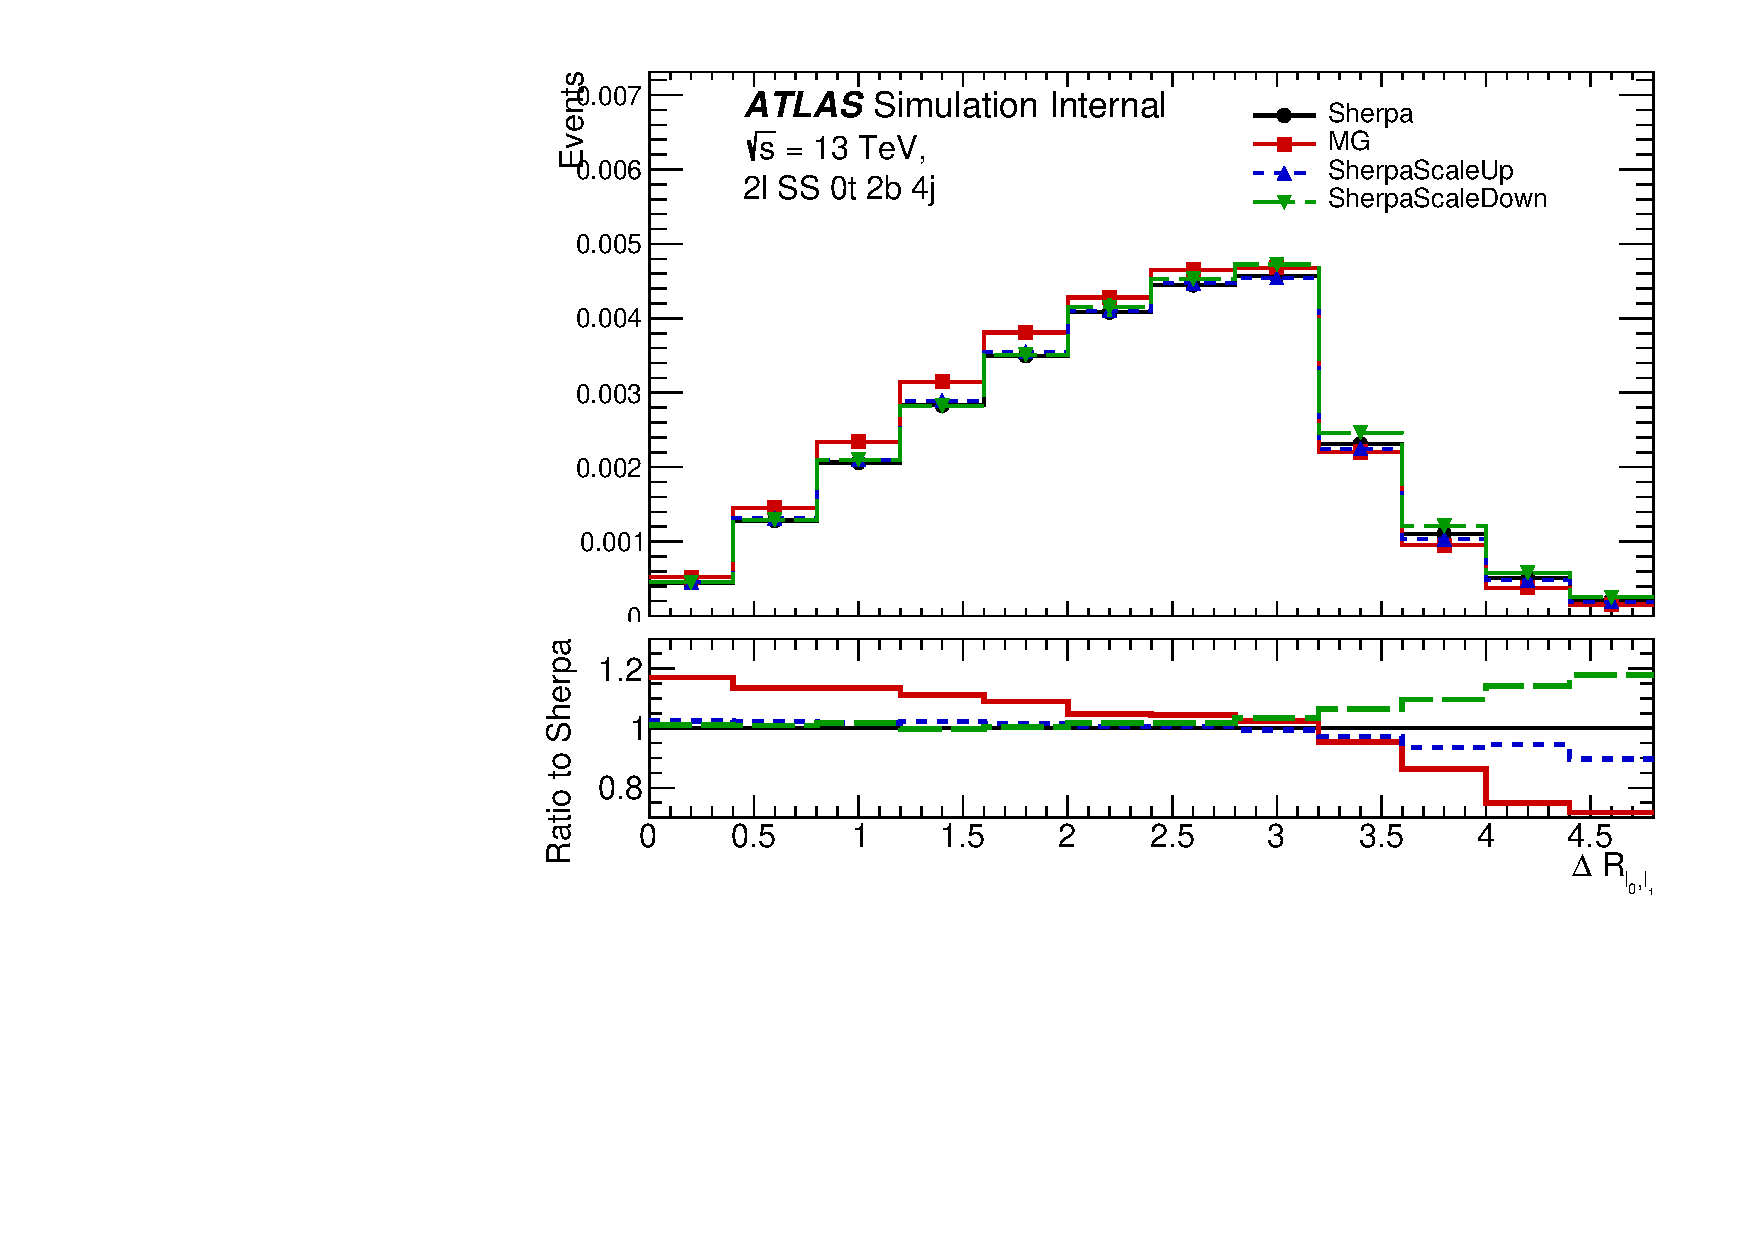
\includegraphics[width=0.45\textwidth]{Plots/ttV/c_Region_1_DRll01}\\
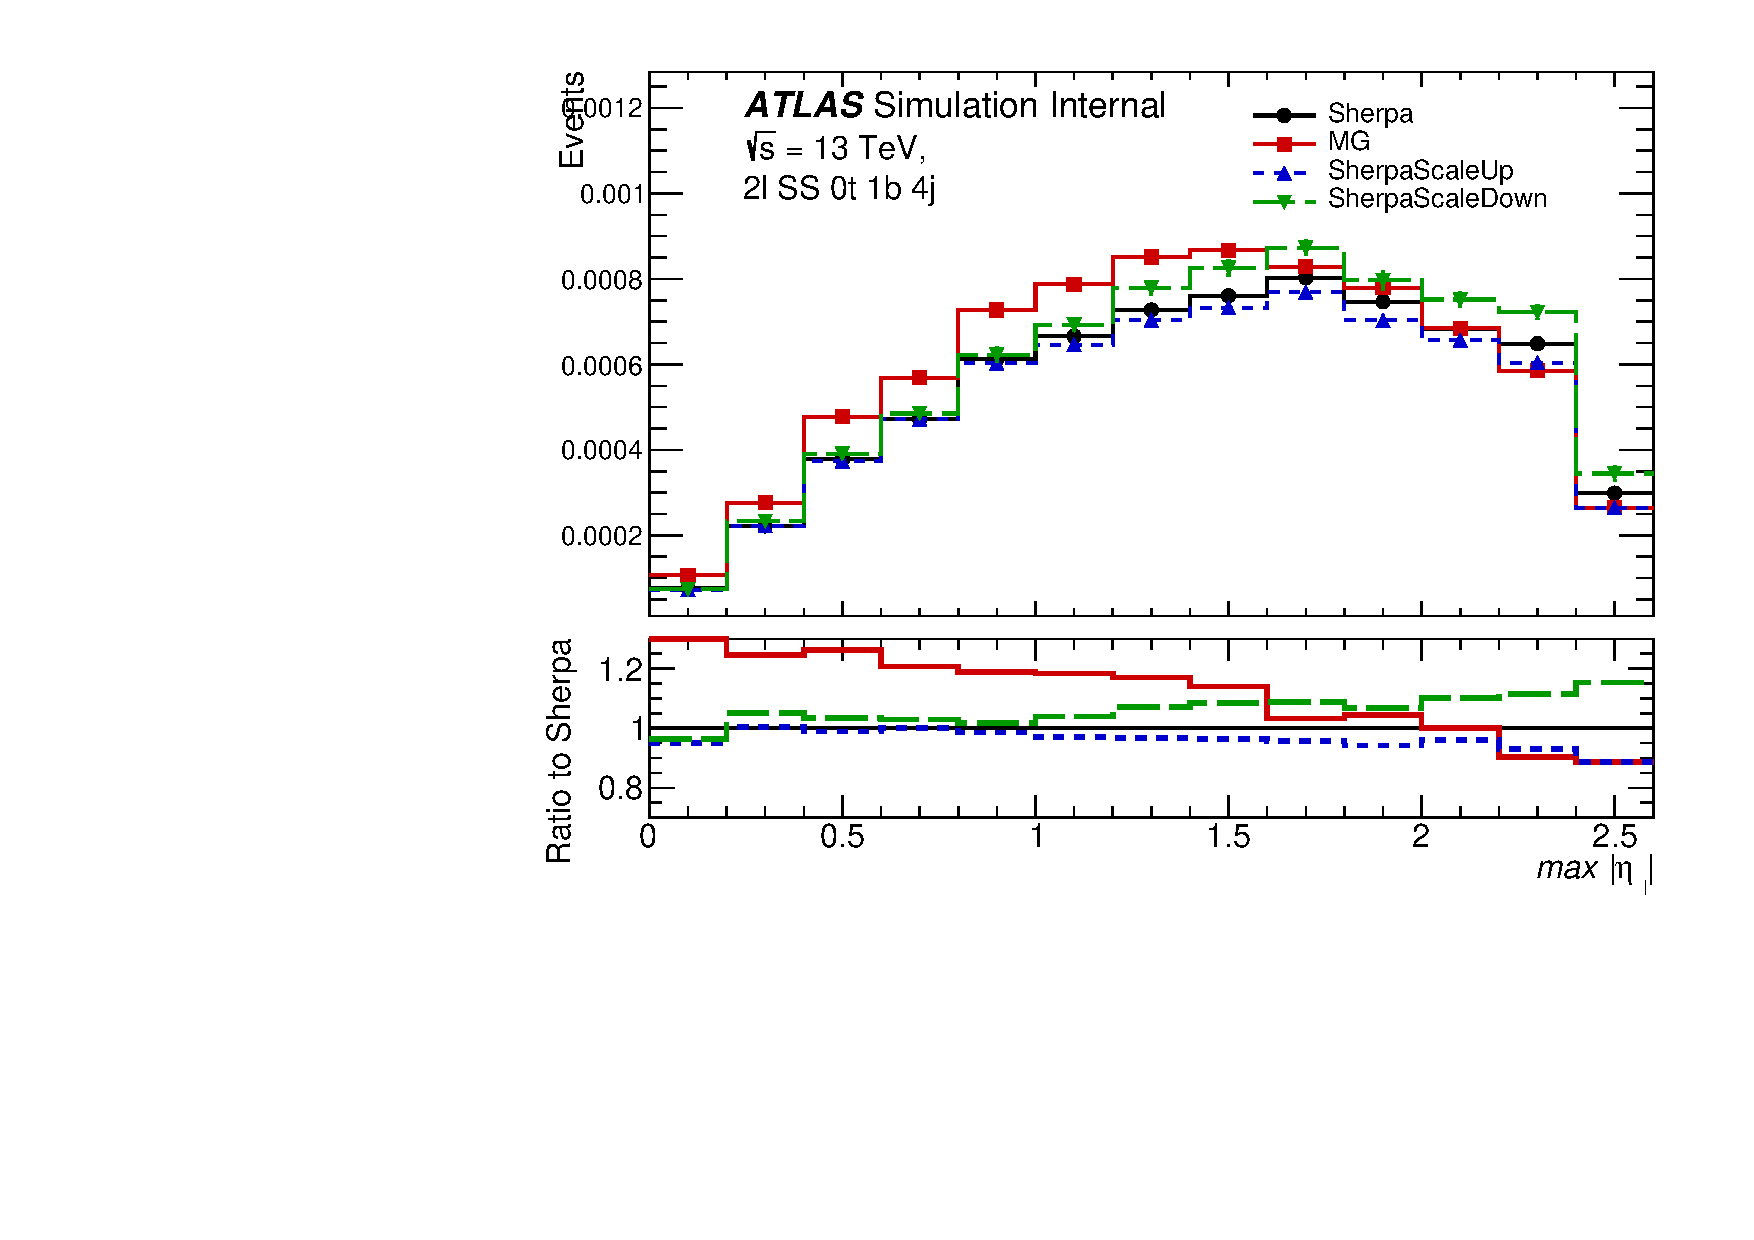
\includegraphics[width=0.45\textwidth]{Plots/ttV/c_Region_0_maxEta_ll} 
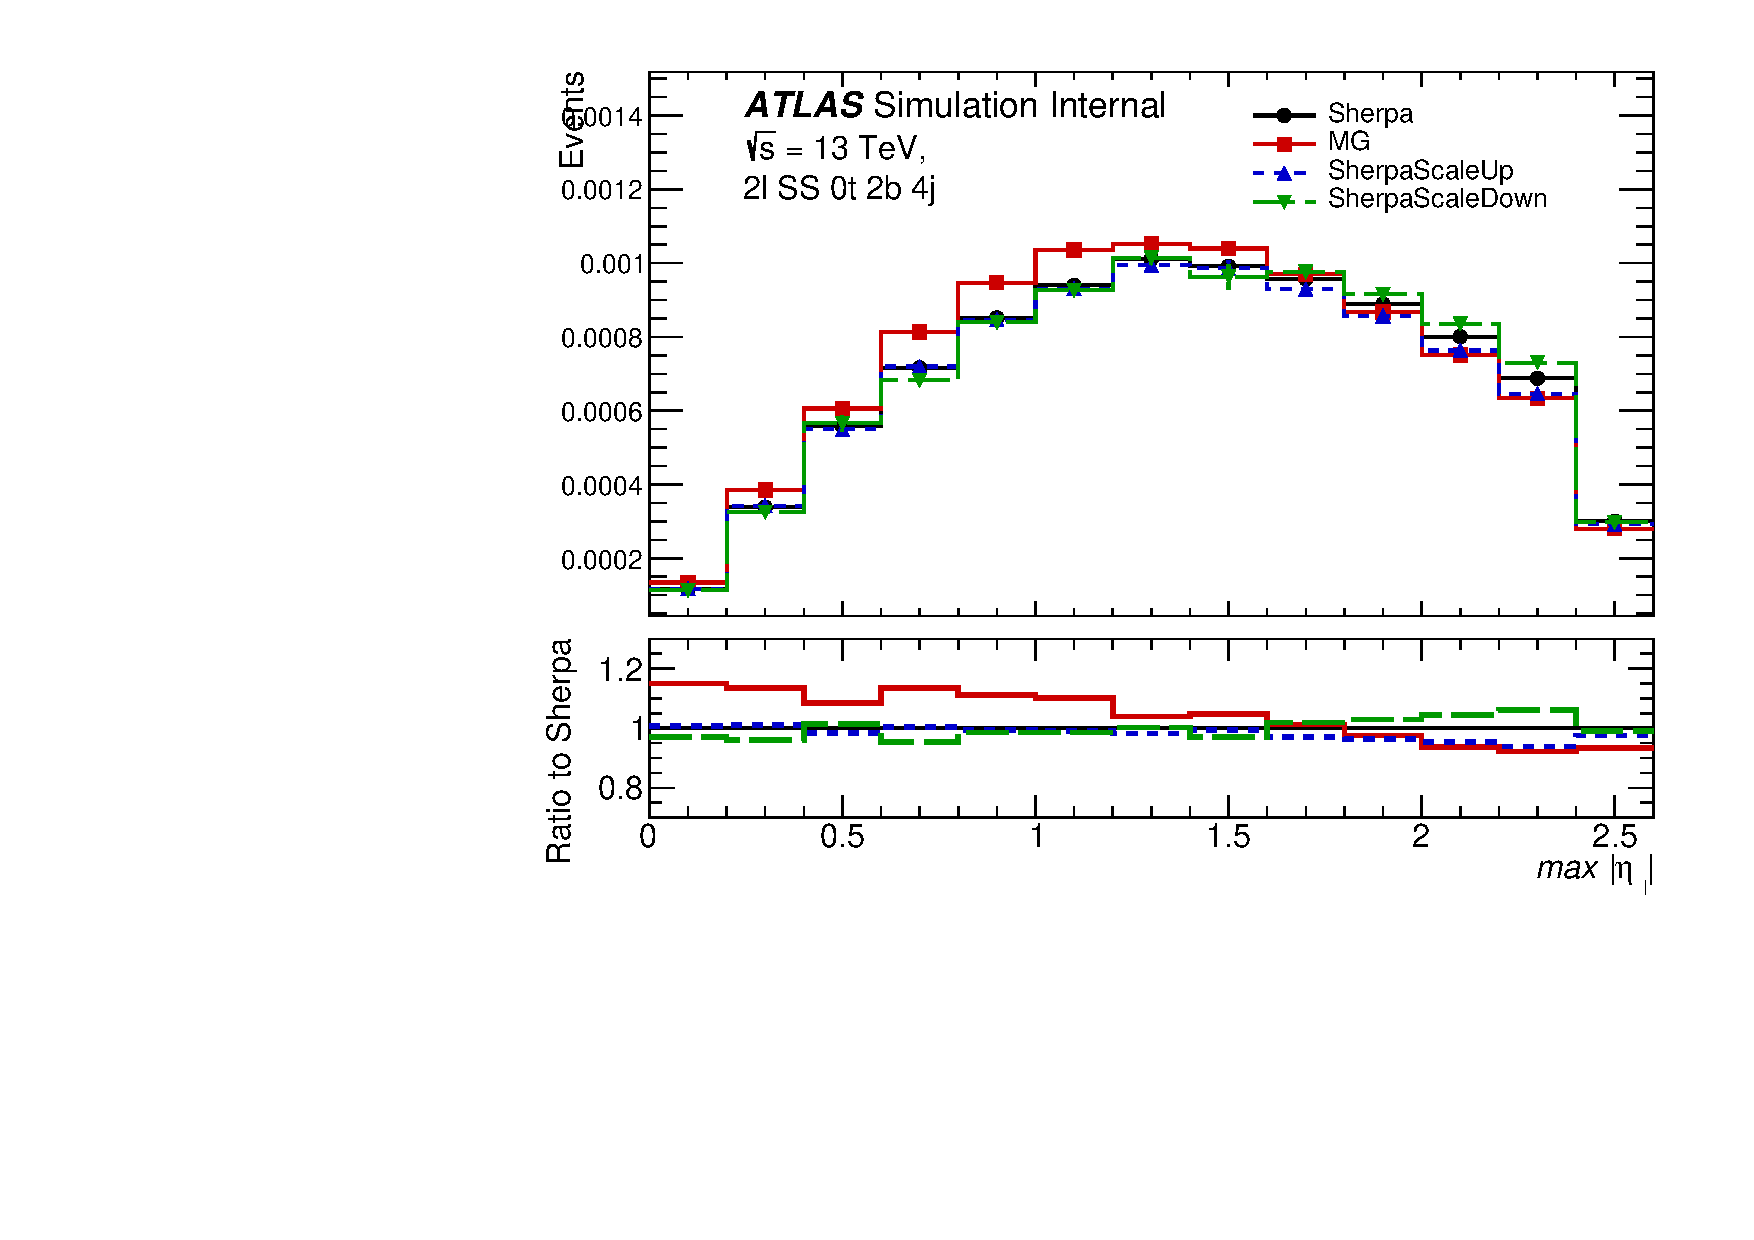
\includegraphics[width=0.45\textwidth]{Plots/ttV/c_Region_1_maxEta_ll}\\
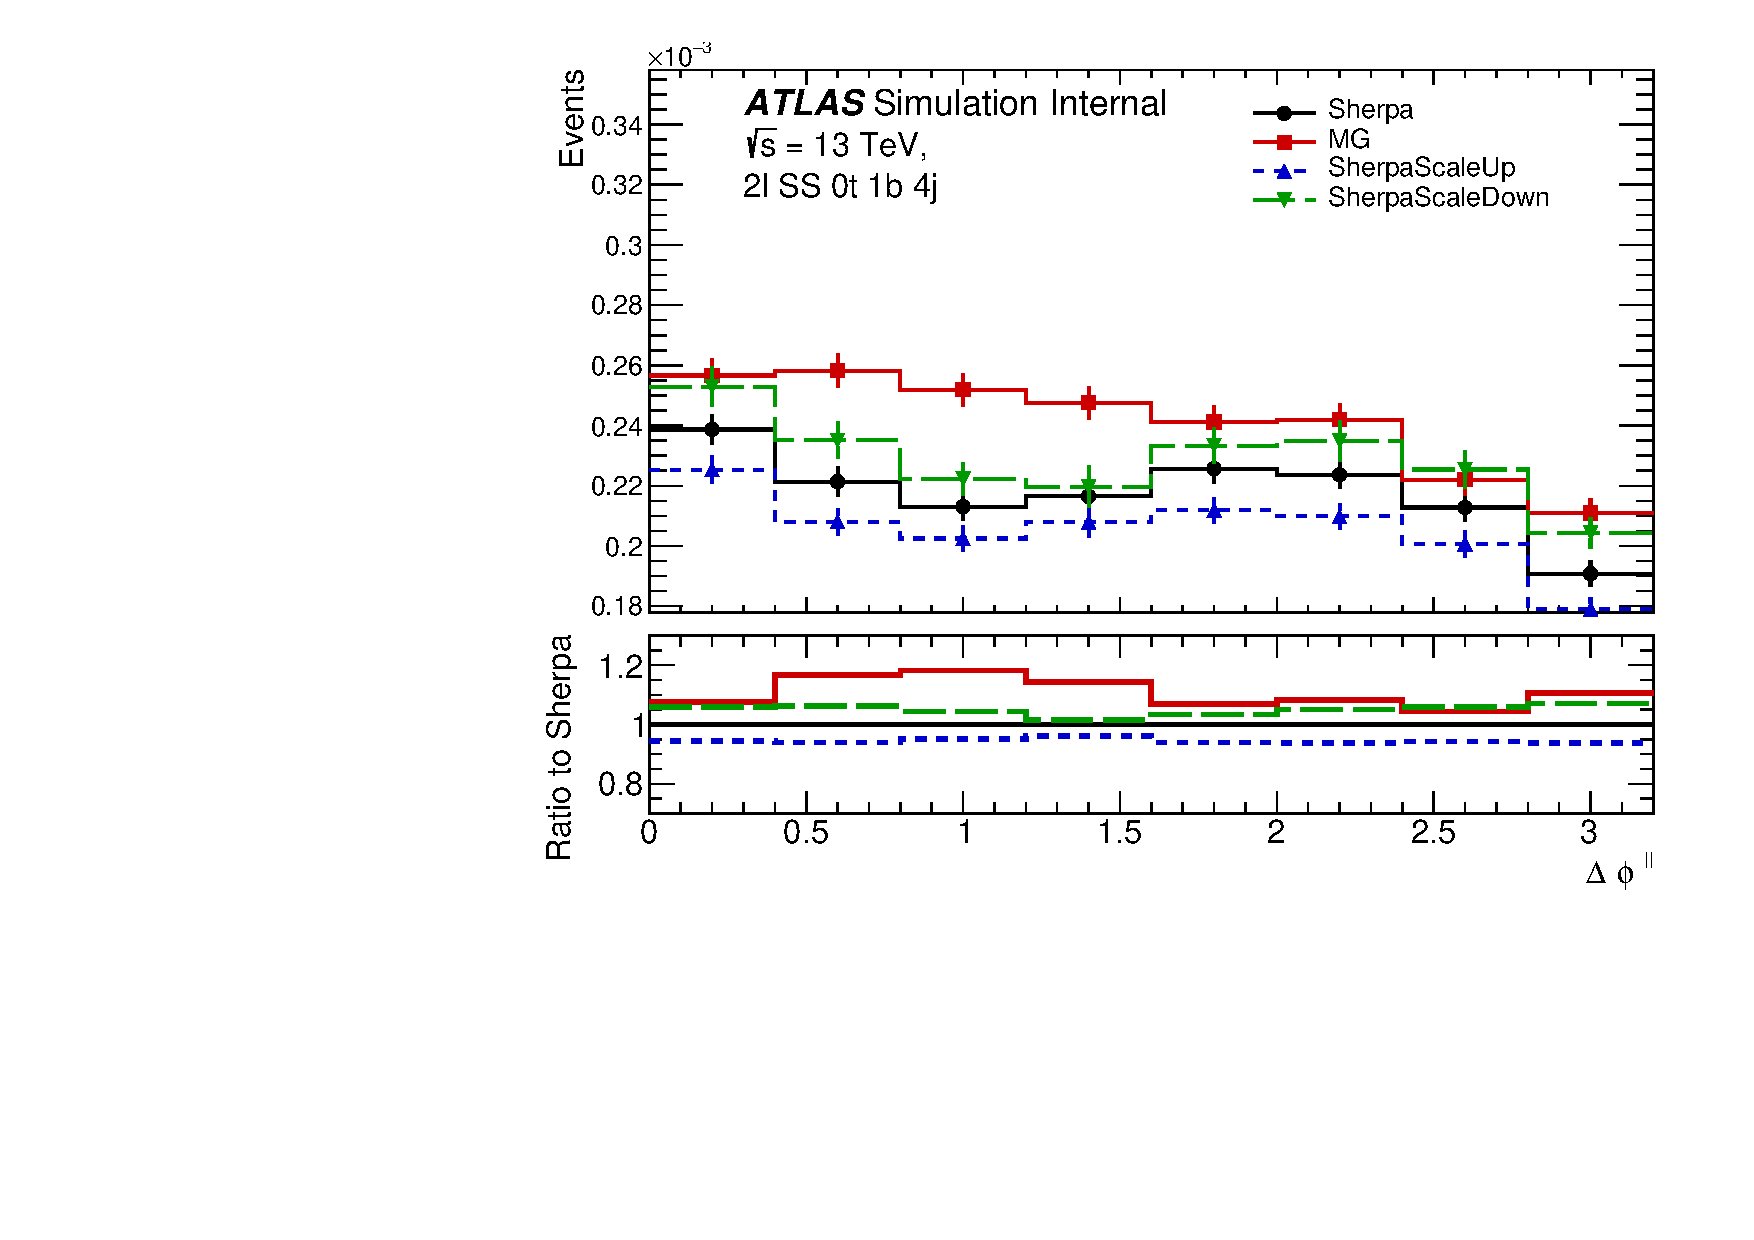
\includegraphics[width=0.45\textwidth]{Plots/ttV/c_Region_0_lep_dPhi} 
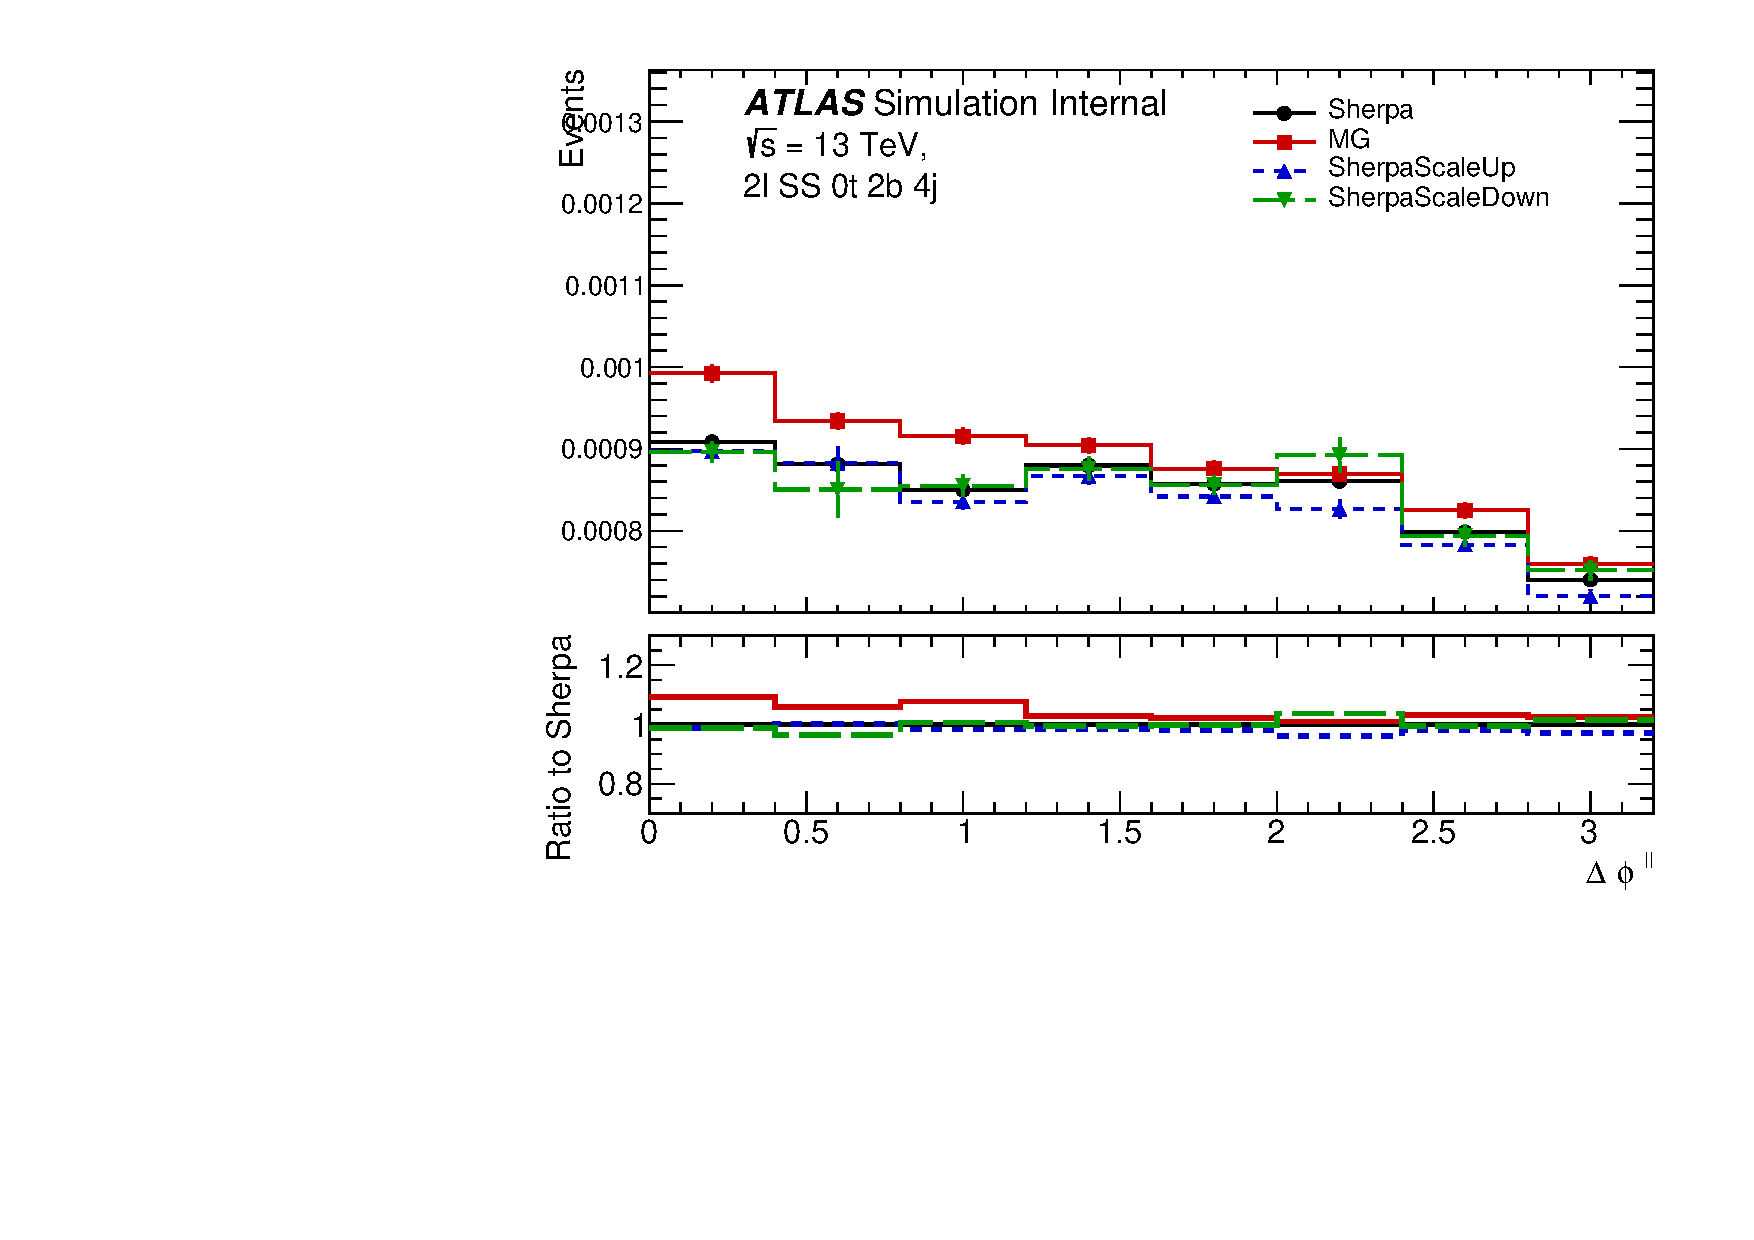
\includegraphics[width=0.45\textwidth]{Plots/ttV/c_Region_1_lep_dPhi} 
  \caption{Distribution of the angular distance between the two leptons (top), maximum between lepton $|\eta_{\ell 0}|$ and $|\eta_{\ell 1}|$ (centre), azimuthal separation between the leptons $\Delta \phi _{\ell \ell }$ (bottom) , for the Region 1 with 1$b$-jet (left) and Region 2 with 2$b$-jets (right) selection requiring four and more jets. Explanation in text.
   \label{ttV:ll_kin}}
\end{figure}
% 



\begin{figure}[!htb]
\centering
	% \hspace{25mm} $DRl_0l_1$  \hspace{20mm} $max|\eta^{\ell\ell}|$\\
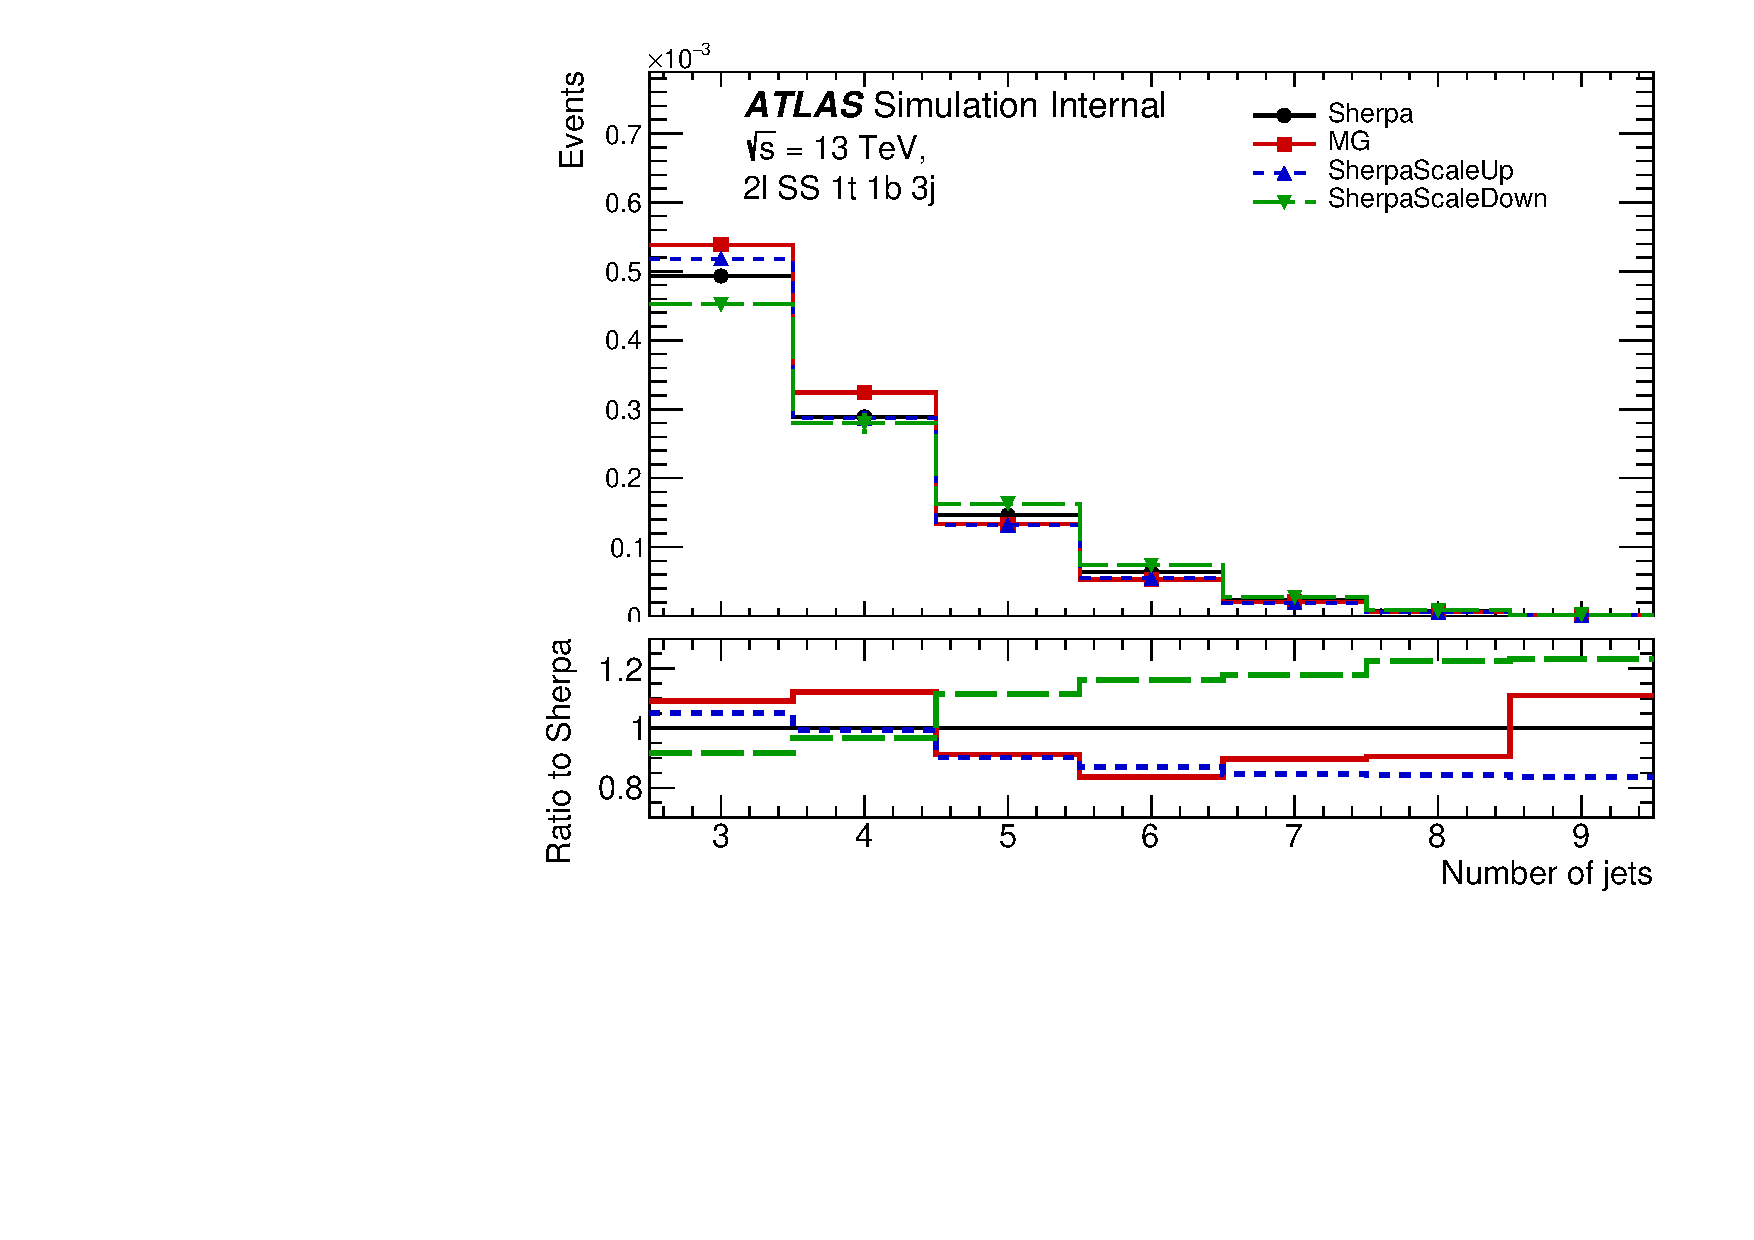
\includegraphics[width=0.45\textwidth]{Plots/ttV/c_Region_4_nJets}
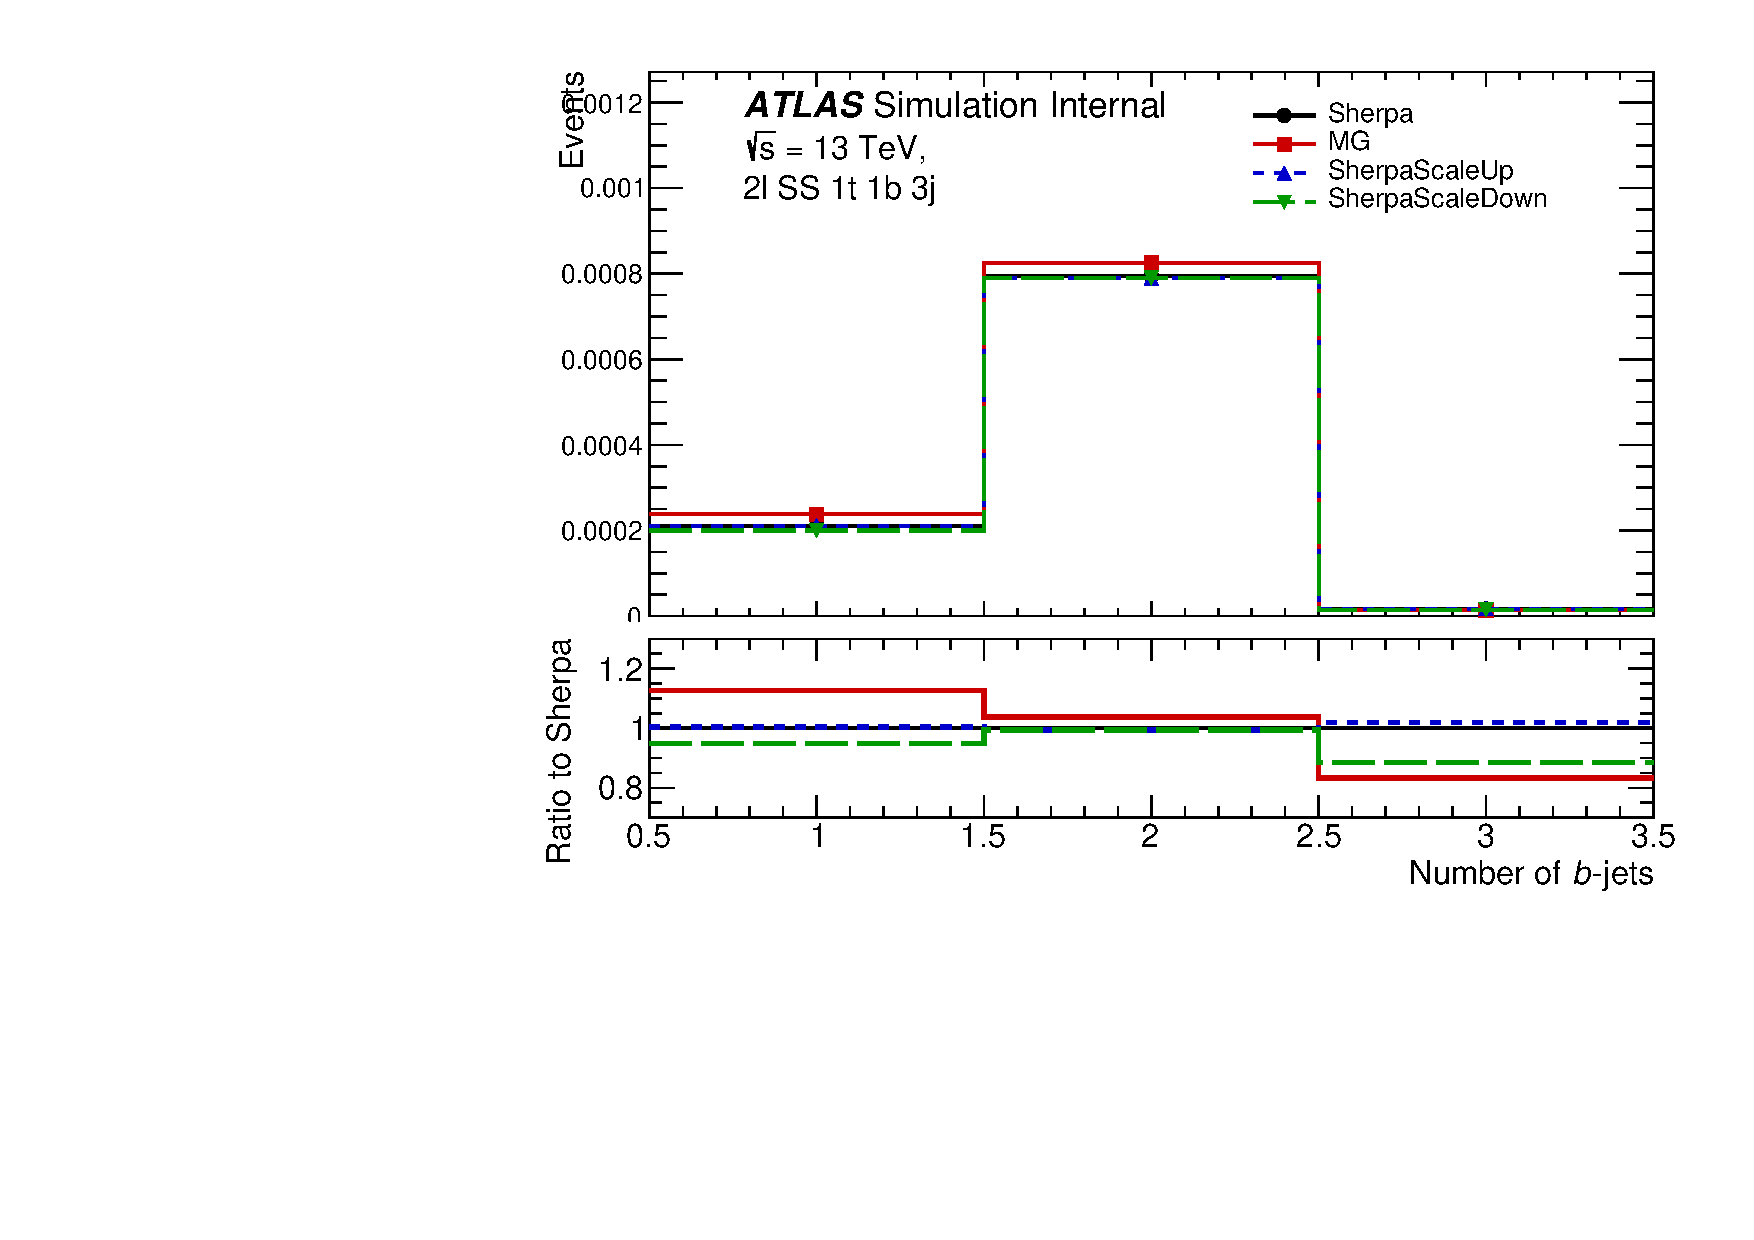
\includegraphics[width=0.45\textwidth]{Plots/ttV/c_Region_4_nBtagJets}\\
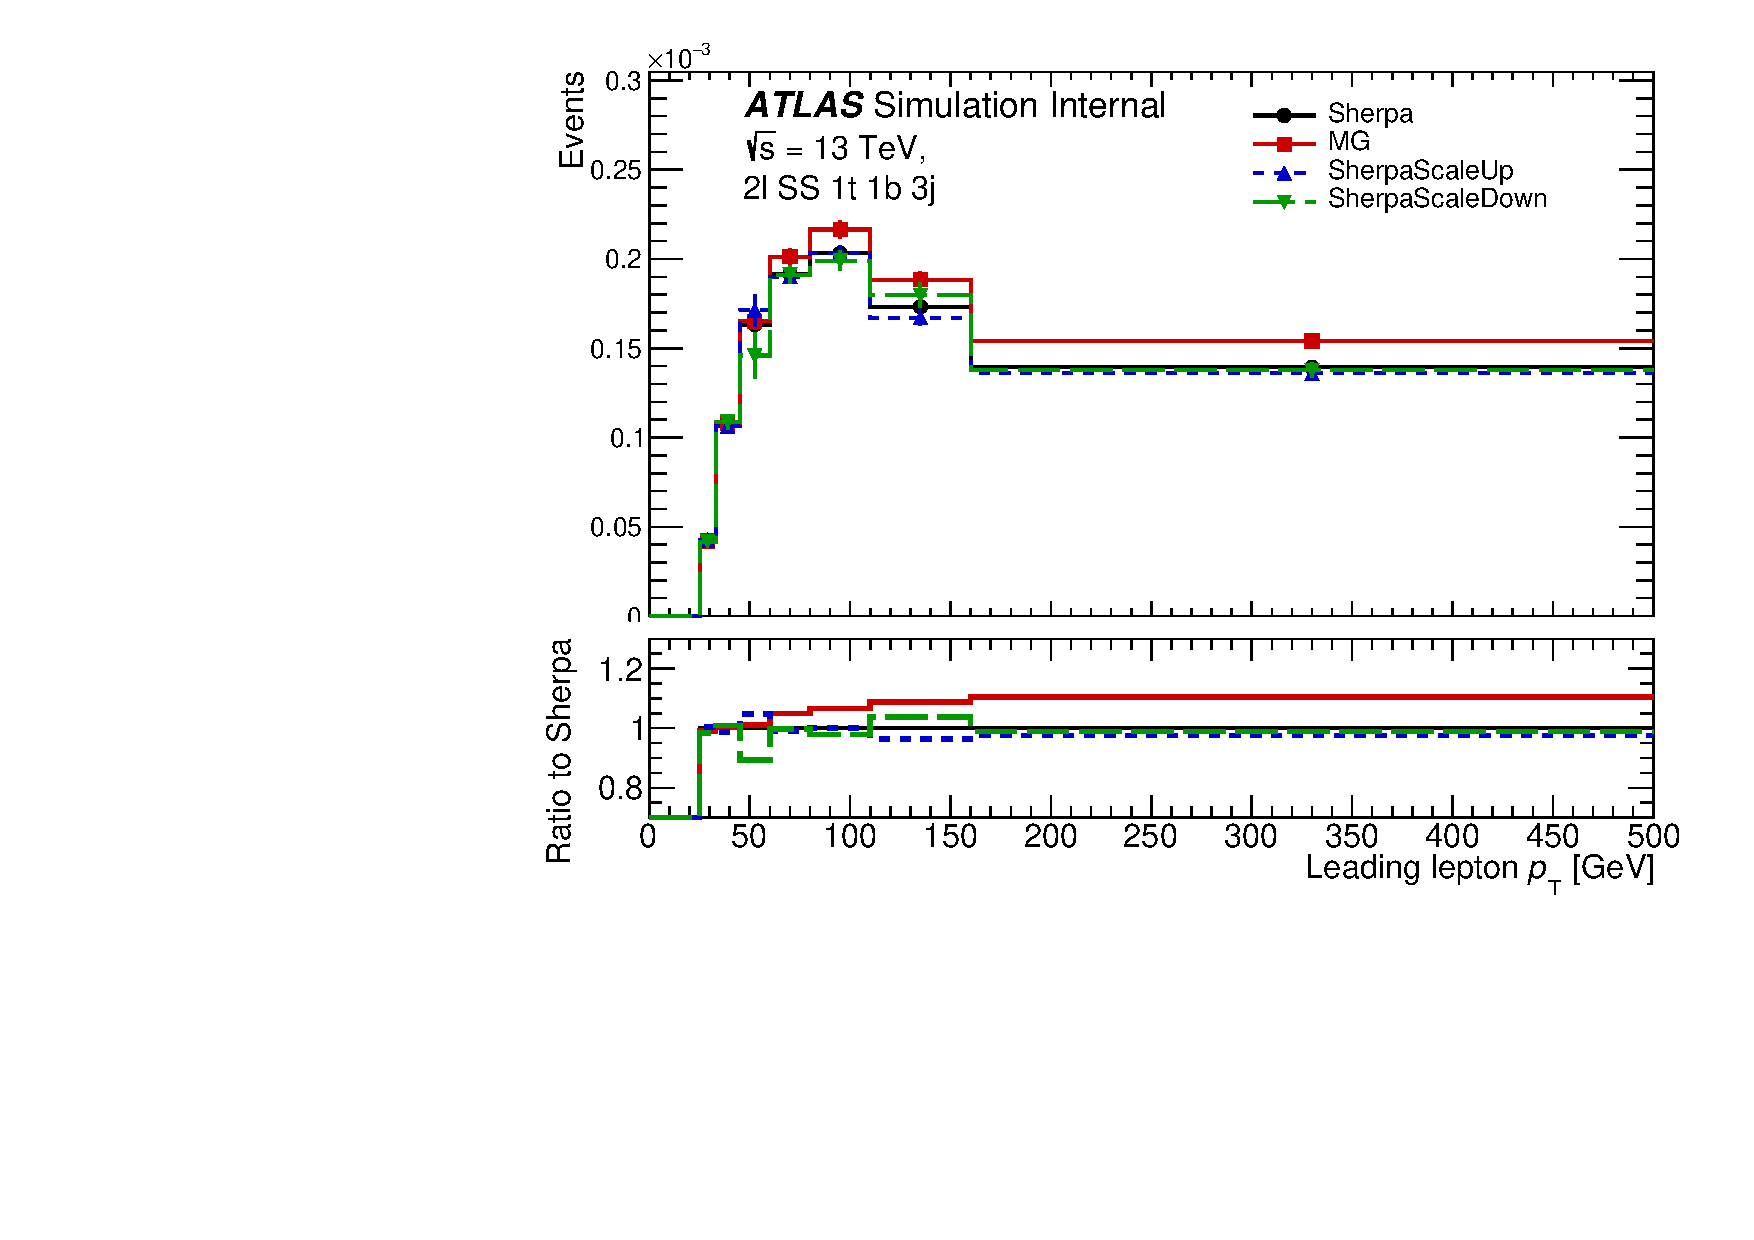
\includegraphics[width=0.45\textwidth]{Plots/ttV/c_Region_4_lep_Pt_0} 
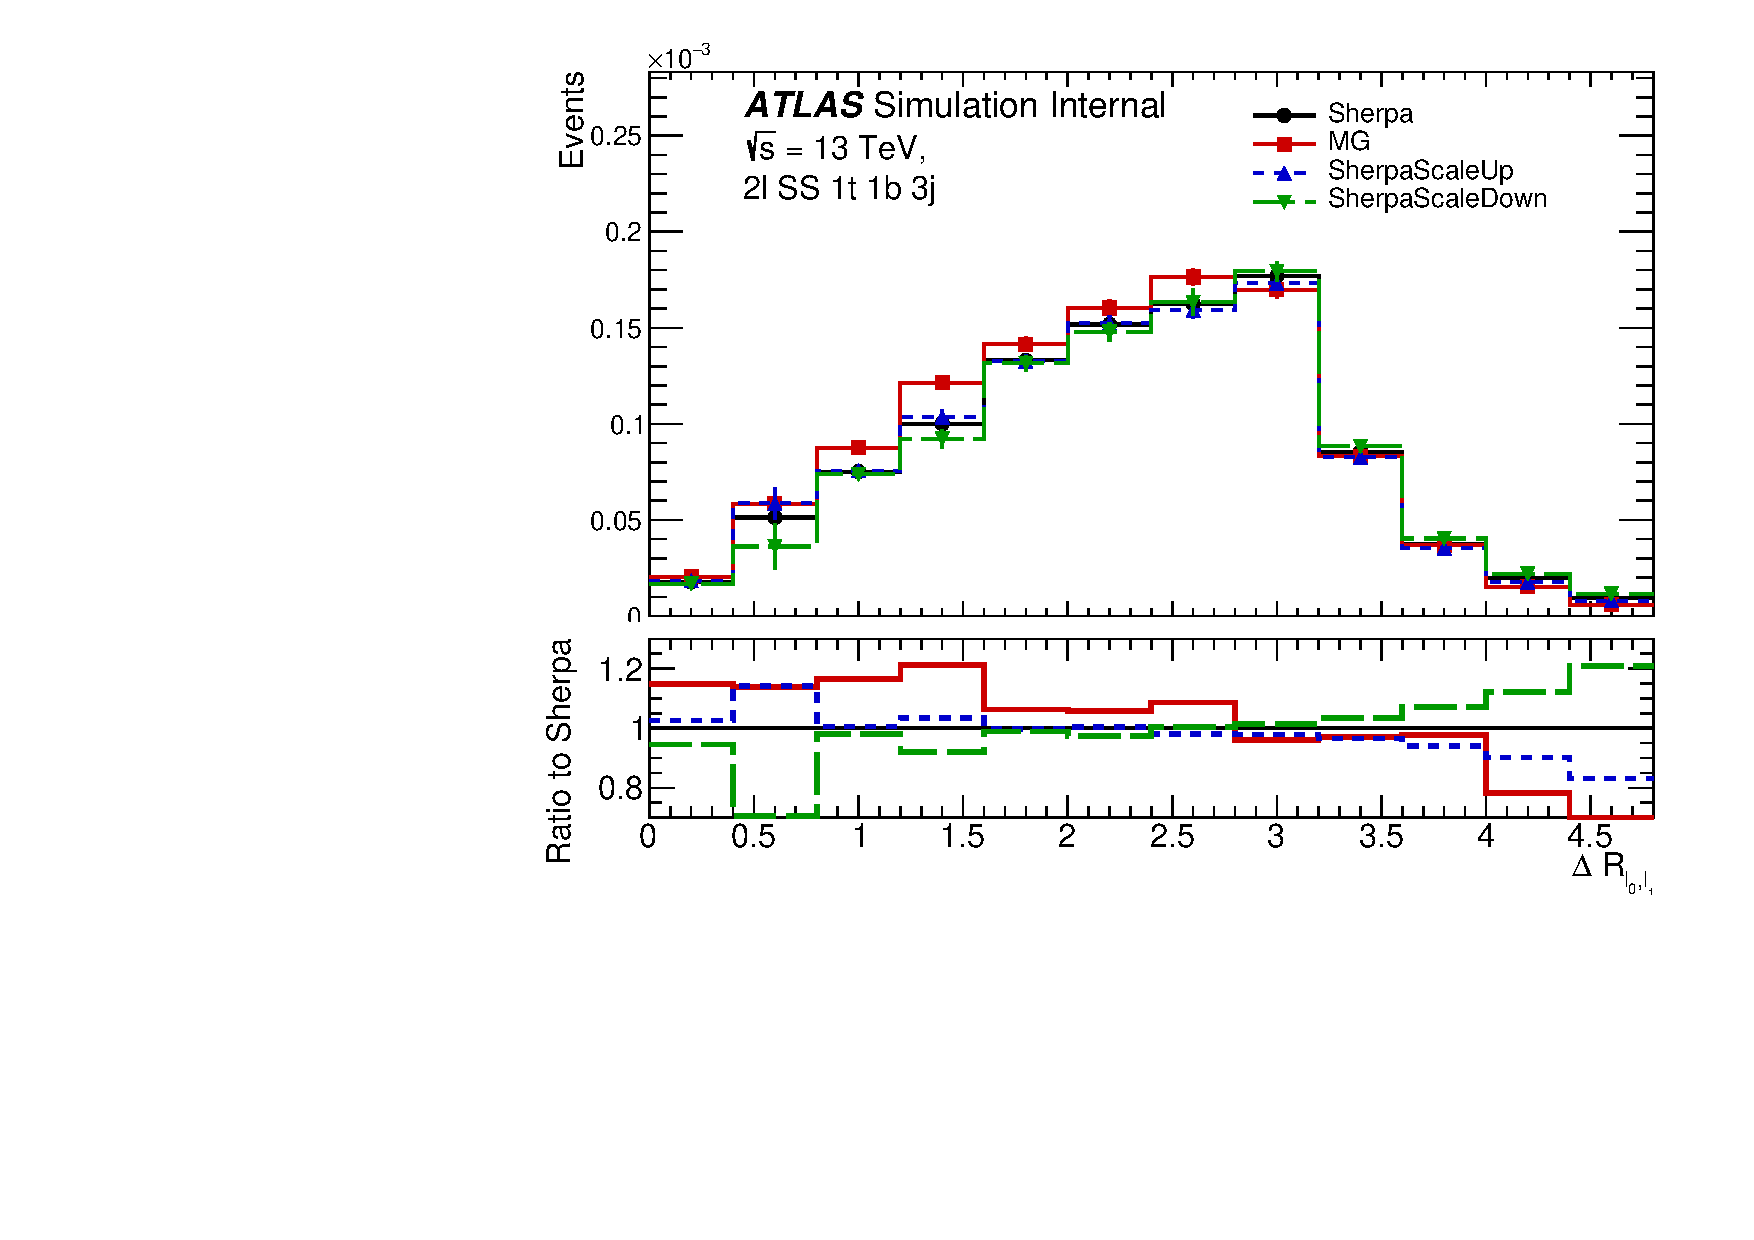
\includegraphics[width=0.45\textwidth]{Plots/ttV/c_Region_4_DRll01}\\
  \caption{Distribution of the the jet multiplicity, number of $b$-jets, the leading lepton transverse momentum and the angular distance between the two leptons  $\Delta R _{\ell \ell }$ for the Region 5 with 1$\tau_{had}$ selection. Explanation in text.
   \label{ttV:tauR_kin}}
\end{figure}
% 


